% General Paper Template created by Adam Green
% Last revised 1/09/18

\documentclass[12pt]{article}

%%%%%%%%%%%%%%%%%%%%%%%%%%
% Standard packages
%%%%%%%%%%%%%%%%%%%%%%%%%%
\usepackage{amsmath,amsfonts,amsthm,amssymb}
\usepackage[margin = 2cm]{geometry}
%\usepackage{siunitx}

%%%%%%%%%%%%%%%%%%%%%%%%%%
% Graphical packages
%%%%%%%%%%%%%%%%%%%%%%%%%%
\usepackage{graphicx}
\usepackage{subfig}
\usepackage{float}
\usepackage{tikz}
%\usepackage{tikz-3dplot}
%\usepackage{pgfplots}

\graphicspath{{Figures/}} % set directory for figures


%%%%%%%%%%%%%%%%%%%%%%%%%%
% Table and Array packages
%%%%%%%%%%%%%%%%%%%%%%%%%%
\usepackage{tabu}
\usepackage{booktabs}
\usepackage{xcolor}


%%%%%%%%%%%%%%%%%%%%%%%%%%
% Citation packages
%%%%%%%%%%%%%%%%%%%%%%%%%%
\usepackage{hyperref}
%\hypersetup{citebordercolor = {0 0.75 0.75}, linkbordercolor = {0 0.75 0.75} }
\hypersetup{allcolors = {0 0.75 0.75}, allbordercolors = {0 0.75 0.75}, filecolor = {0 0.75 0.75}, linkbordercolor = {0 0.75 0.75} }
\usepackage{cleveref}

%%%%%%%%%%%%%%%%%%%%%%%%%%
% Text Formatting packages
%%%%%%%%%%%%%%%%%%%%%%%%%%
\usepackage{multicol}
\usepackage{parskip} 
\usepackage{indentfirst} 
	\setlength{\parindent}{14pt}
\usepackage{fancyhdr}
%	\pagestyle{fancy}
\usepackage{enumerate}
\usepackage{wrapfig}
\usepackage{lipsum}
\usepackage{caption}
	\captionsetup{format=hang, justification = raggedright, singlelinecheck=false}
	

%%%%%%%%%%%%%%%%%%%%%%%%%%
% Custom Commands
%%%%%%%%%%%%%%%%%%%%%%%%%%
\renewcommand{\deg}{^\circ} % Degree Symbol (only in math mode)
\renewcommand{\vec}[1]{\mathbf{#1}} % boldface vectors




\newcommand{\red}[1]{\textbf{\textcolor{red}{#1}}} % My standard commenting style
\newcommand{\scap}[1]{\textsc{\makeLowercase{#1}}} % Makes caps small so it doesnt SHOUT

\newcommand{\Ylm}[2]{\mathrm{Y}^{#1}_{#2}}

% Math commands, first and second order partials, Laplacian
\newcommand{\evaluate}{\Bigr\rvert}
\newcommand{\ppd}[1]{\frac{\partial}{\partial#1}}
\newcommand{\ppsd}[1]{\frac{\partial^2}{\partial #1^2}}
\newcommand{\ppnd}[2]{\frac{\partial #1}{\partial #2}}
\newcommand{\ppsnd}[2]{\frac{\partial^2 #1}{\partial #2^2}}
\newcommand{\lap}{\nabla^2}

% Quantum bra- ket- commands
\newcommand{\bra}[1]{\langle #1 |}
\newcommand{\ket}[1]{| #1 \rangle}
\newcommand{\bracket}[2]{\langle #1 | #2 \rangle}

% Redfine equation and figure references to include "Eqn. ()" and "Fig. _"
\newcommand{\figref}[1]{Fig.\ \ref{#1}}
\let\originaleqref=\eqref
\renewcommand{\eqref}{Eqn.\ \originaleqref}


% Custom matrix spacing
% Syntax: \begin{matrix}[scale]
\makeatletter
\renewcommand*\env@matrix[1][\arraystretch]{%
	\edef\arraystretch{#1}%
	\hskip -\arraycolsep
	\let\@ifnextchar\new@ifnextchar
	\array{*\c@MaxMatrixCols c}}
\makeatother

\newcommand{\email}[1]{\href{mailto:#1}{#1}}
\newenvironment{institutions}[1][2em]{\begin{list}{}{\setlength\leftmargin{#1}\setlength\rightmargin{#1}}\item[]}{\end{list}}


\begin{document}

	
%%%%%%%%%%%%%%%%%%%%%%%%%%%
% Title
%%%%%%%%%%%%%%%%%%%%%%%%%%%	
\begin{center}

	{\huge \bf Quantum Analogs}
	
	\vspace{0.5cm}
	
	\textbf{Adam Green}, \textbf{Guillermo Acuna}\\
	
	\texttt{\footnotesize \email{agree019@ucr.edu}},
	\texttt{\footnotesize \email{gacun002@ucr.edu}}
	
	\vspace{0.5cm}
	
	
	\begin{institutions}[2.25cm]
		\footnotesize
		{\it 
			Department of Physics \& Astronomy, 
			University of  California, Riverside, 
			{CA} 92521	    
		}    
	\end{institutions}

	\vspace{0.5cm}
	
\end{center}

%%%%%%%%%%%%%%%%%%%%%%%%%%%
% Abstract
%%%%%%%%%%%%%%%%%%%%%%%%%%%	
	\vspace{0.5cm}

\begin{abstract}
Abstract Things	
\end{abstract}
	
	\section{Introduction}
	Often times in physics, the specific mathematical equations used to represent physical systems can become system-independent under special circumstances. In other words, the same equations can be used to describe very different systems. One intriguing example is a parallel between the Shcr\"odinger equation and the wave equation. Both equations describe a sort of ``wave.'' In the Schr\"odinger equation, the ``wave'' is not a physical wave, but a probability wave. In the case of the wave equation, the wave is a physical pressure wave. Nonetheless, under special circumstances, these two equations can be modeled the same way.
	
	In this experiment, we model the wavefunction of the Hydrogen atom with a physical pressure wave inside a hollow spherical cavity. This is possible because the conditions inside the spherical cavity mimic the conditions of a Hydrogen atom and the equations which describe the wavefunction and pressure wave have the same solution. We will begin by analyzing the solutions to both the Schr\"odinger equation and the wave equation.

	
	\hrulefill
	
	The Schr\"odinger equation is used to describe the time-evolution of a quantum mechanical system and is given by:
	\begin{equation}
	\label{schrodingerEqn1}
		i\hbar\ppnd{\psi}{t} = \left[-\frac{\hbar^2}{2m}\lap+ V(\vec{r},t)\right] \psi
	\end{equation}
	where $\psi$ is a complex wavefunction which has temporal and spatial dependence, $\psi = \psi{(\vec{r},t)}$, and $V(\vec{r},t)$ is a time and space dependent potential.
	
	When the potential is time-independent, as in our case for the Coulomb potential $V = V(\vec{r})$, stationary states form in which the energy of the wavefunction remains constant and the Schr\"odinger equations reduces to:
	\begin{equation}
	\label{schrodingerEqn2}
		E \psi = \left[-\frac{\hbar^2}{2m}\lap + V(\vec{r})\right] \psi
	\end{equation}
	For our case, the potential will be the Coulomb potential $V(r) = -e^2/r$. Taking advantage of spherical symmetry of the potential and spherical laplacian, we may rewrite the Schr\"odinger equation in spherical coordinates:
	\begin{equation}
	\label{schroderEqnSphere}
		E \psi = -\frac{e^2}{r} + \frac{\hbar}{2m} \left[ \frac{1}{r^2} \ppd{r}r^2 \ppd{r} + \frac{1}{r^2\sin(\theta)}\ppd{\theta}\sin(\theta)\ppd{\theta} + \frac{1}{r^2\sin^2(\theta)} \ppsd{\varphi} \right] \psi 
	\end{equation}
	where the first term is the Coulomb potential. We may solve \eqref{schroderEqnSphere} with separation of variables, in which case the the solution admits the following form:
	\begin{equation}
		\psi(r,\theta,\varphi) = \mathrm{Y}_\ell^m(\theta,\varphi) \, \mathrm{R}(r)
	\end{equation}
	The entire angular dependence of \eqref{schroderEqnSphere} is contained in the spherical harmonics $\mathrm{Y}_\ell^m(\theta,\varphi)$. Here, $\ell$ and $m$ are the two quantum numbers representing angular momentum and magnetic spin respectively. Similarly, the entire radial dependence of \eqref{schroderEqnSphere} is contained in $\mathrm{R}(r)$.
	
	The spherical harmonics $\mathrm{Y}_\ell^m(\theta,\varphi)$ satisfy:
	\begin{equation}
	\label{sphericalHarmonic}
		-\left[ \frac{1}{\sin(\theta)}\ppd{\theta}\sin(\theta)\ppd{\theta} + \frac{1}{\sin^2(\theta)} \ppsd{\varphi} \right] \, \mathrm{Y}_\ell^m = \ell(\ell+1)\mathrm{Y}_\ell^m
	\end{equation}
	and admit solutions which are proportional to the Legendre polynomials $P_\ell^m(\cos(\theta))$ and a complex exponential:
	\begin{equation}
		\mathrm{Y}_\ell^m(\theta,\varphi) \propto P_\ell^m(\cos(\theta))e^{im\varphi}
	\end{equation}
	\red{the complex exponential however is not physical since it represents a quantum phase which is never observable}
	
	The radial solution $\mathrm{R}(r)$ satisfies:
	\begin{equation}
	\label{radialSoln}
		- \frac{\hbar}{2m} \left[ \frac{1}{r} \ppsd{r}r + \frac{\ell(\ell+1)}{r^2} + \frac{e^2}{r} \right] \mathrm{R}(r) = E \, \mathrm{R}(r)
	\end{equation}
	
	\hrulefill
	
	We will now shift our attention to the spherical acoustic resonator which contains a pressure wave $\rho$ whose time-evolution is described by the wave equation:
	\begin{equation}
		\label{waveEqn1}
		\ppsnd{\rho}{t} = v^2 \, \lap\rho
	\end{equation}
	where $v$ is the velocity of the wave, and the quantity $\rho = \rho(\vec{r},t)$ represents the wave. To solve \eqref{waveEqn1}, we assume the following functional form for the pressure wave:
	\begin{equation}
	\label{waveSoln}
		\rho(\vec{r},t) = \mathrm{P}(\vec{r})\cos(\omega t)
	\end{equation}
	in which case, the wave equation reduces to the time-independent Helmholtz equation:
	\begin{equation}
	\label{helmholtzEqn}
		-\omega^2 \mathrm{P} = \lap \mathrm{P}
	\end{equation}
	We pause here to draw a parallel between the Schr\"odinger equation, \eqref{schrodingerEqn2}, and the time-independent Helmholtz equation, \eqref{helmholtzEqn}. Up to the addition of the the Coulomb potential in the Schr\"odinger equation, the two equations have the same differential form, and we expect similar solutions.
	
	Proceeding in a similar fashion to the Schr\"odinger analysis, we take advantage of the spherical symmetry of the cavity and write \eqref{helmholtzEqn} in spherical coordinates:
	\begin{equation}
	\label{helmholtsSphere}
		\frac{\omega^2}{v^2} \mathrm{P} = \left[ -\frac{1}{r^2} \ppd{r}r^2\ppd{r} - \frac{1}{r^2\sin(\theta)}\ppd{\theta}\sin(\theta)\ppd{\theta} -\frac{1}{r^2\sin^2(\theta)} \ppsd{\varphi} \right] \mathrm{P}
	\end{equation}
	Again, up to the addition of the Coulomb potential, the spherical Helmholtz equation, \eqref{helmholtsSphere}, has the same form as the spherical Schr\"odinger equation,  \eqref{schroderEqnSphere}, so we expect similar behavior of the solutions.

	We proceed in the same fashion and assume a separable solution to \eqref{helmholtsSphere} which takes the form:
	\begin{equation}
		\mathrm{P}(r,\theta,\varphi) = \mathrm{Y}_\ell^m(\theta,\varphi) \mathrm{F}(r)
	\end{equation}
	where the entire angular dependence of the pressure wave is contained in the spherical harmonics $\mathrm{Y}_\ell^m$ just as the case with the Schr\"odinger equation. However, the radial component of the pressure wave obeys a slightly modified differential equation compared to the case of the Hydrogen atom:
	\begin{equation}
		\left[ -\ppsd{r} - \frac{2}{r}\ppd{r} + \frac{\ell(\ell+1)}{r^2} \right] \mathrm{F} = \frac{\omega^2}{v^2}\mathrm{F}
	\end{equation}
		
	Since the Coulomb potential has no angular dependence, it does affect the angular solutions of  either the Schr\"odinger equation or the Helmholtz equation and the angular dependences are identical. 
	
	\red{Talk about energies}
	
	\red{Talk about degeneracies}
		
	
	
		
	\section{Experimental Procedure}
	
		\subsection{Experiment Setup}
		This experiment utilized the \emph{Quantum Analogs Controller} seen in \figref{QAController}. The ``Sine Wave Input'' on the controller is connected to the signal generator and provides the frequency of the signal inside the cavity. The ``Speaker Output'' is connected to the speaker on the cavity. The microphone from the cavity is connected to the ``Microphone Input'' on the device. This reads the signal from the cavity into the controller. The ``A/C Monitor'' port is connected to channel 2 on our oscilloscope. This is the output of the microphone from inside the cavity. Finally, we connect the ``Detector Output'' on the controller to a multimeter set to read DC voltage. The controller converts the AC microphone signal to its envelope and outputs it as a DC signal to ``Detector Output.'' A full view of our lab bench can be used for reference in \figref{experiment}.
		
		The main apparatus for this experiment is the spherical cavity. The microphone and speaker configuration inside the cavity is characterized by the \emph{cavity angle} $\alpha$. When spherical symmetry is present, the conversion from the cavity angle $\alpha$ to polar angle $\theta$ is:
		\begin{equation}
		\label{alpha2theta}
		\cos(\theta) = \frac{1}{2}\cos(\alpha) - \frac{1}{2}
		\end{equation}
		In Appendix A, \figref{ThetaAlpha} shows the relation between cosine of the polar angle $\theta$ and the cavity angle $\alpha$. When the spherical symmetry is broken however, the system is quantized about the $\vec{z}$ axis perpendicular to the table, and the cavity angle is equal to the azimuthal angle $\varphi$.
		
%
%		\begin{wrapfigure}{l}{0.5\textwidth}
%		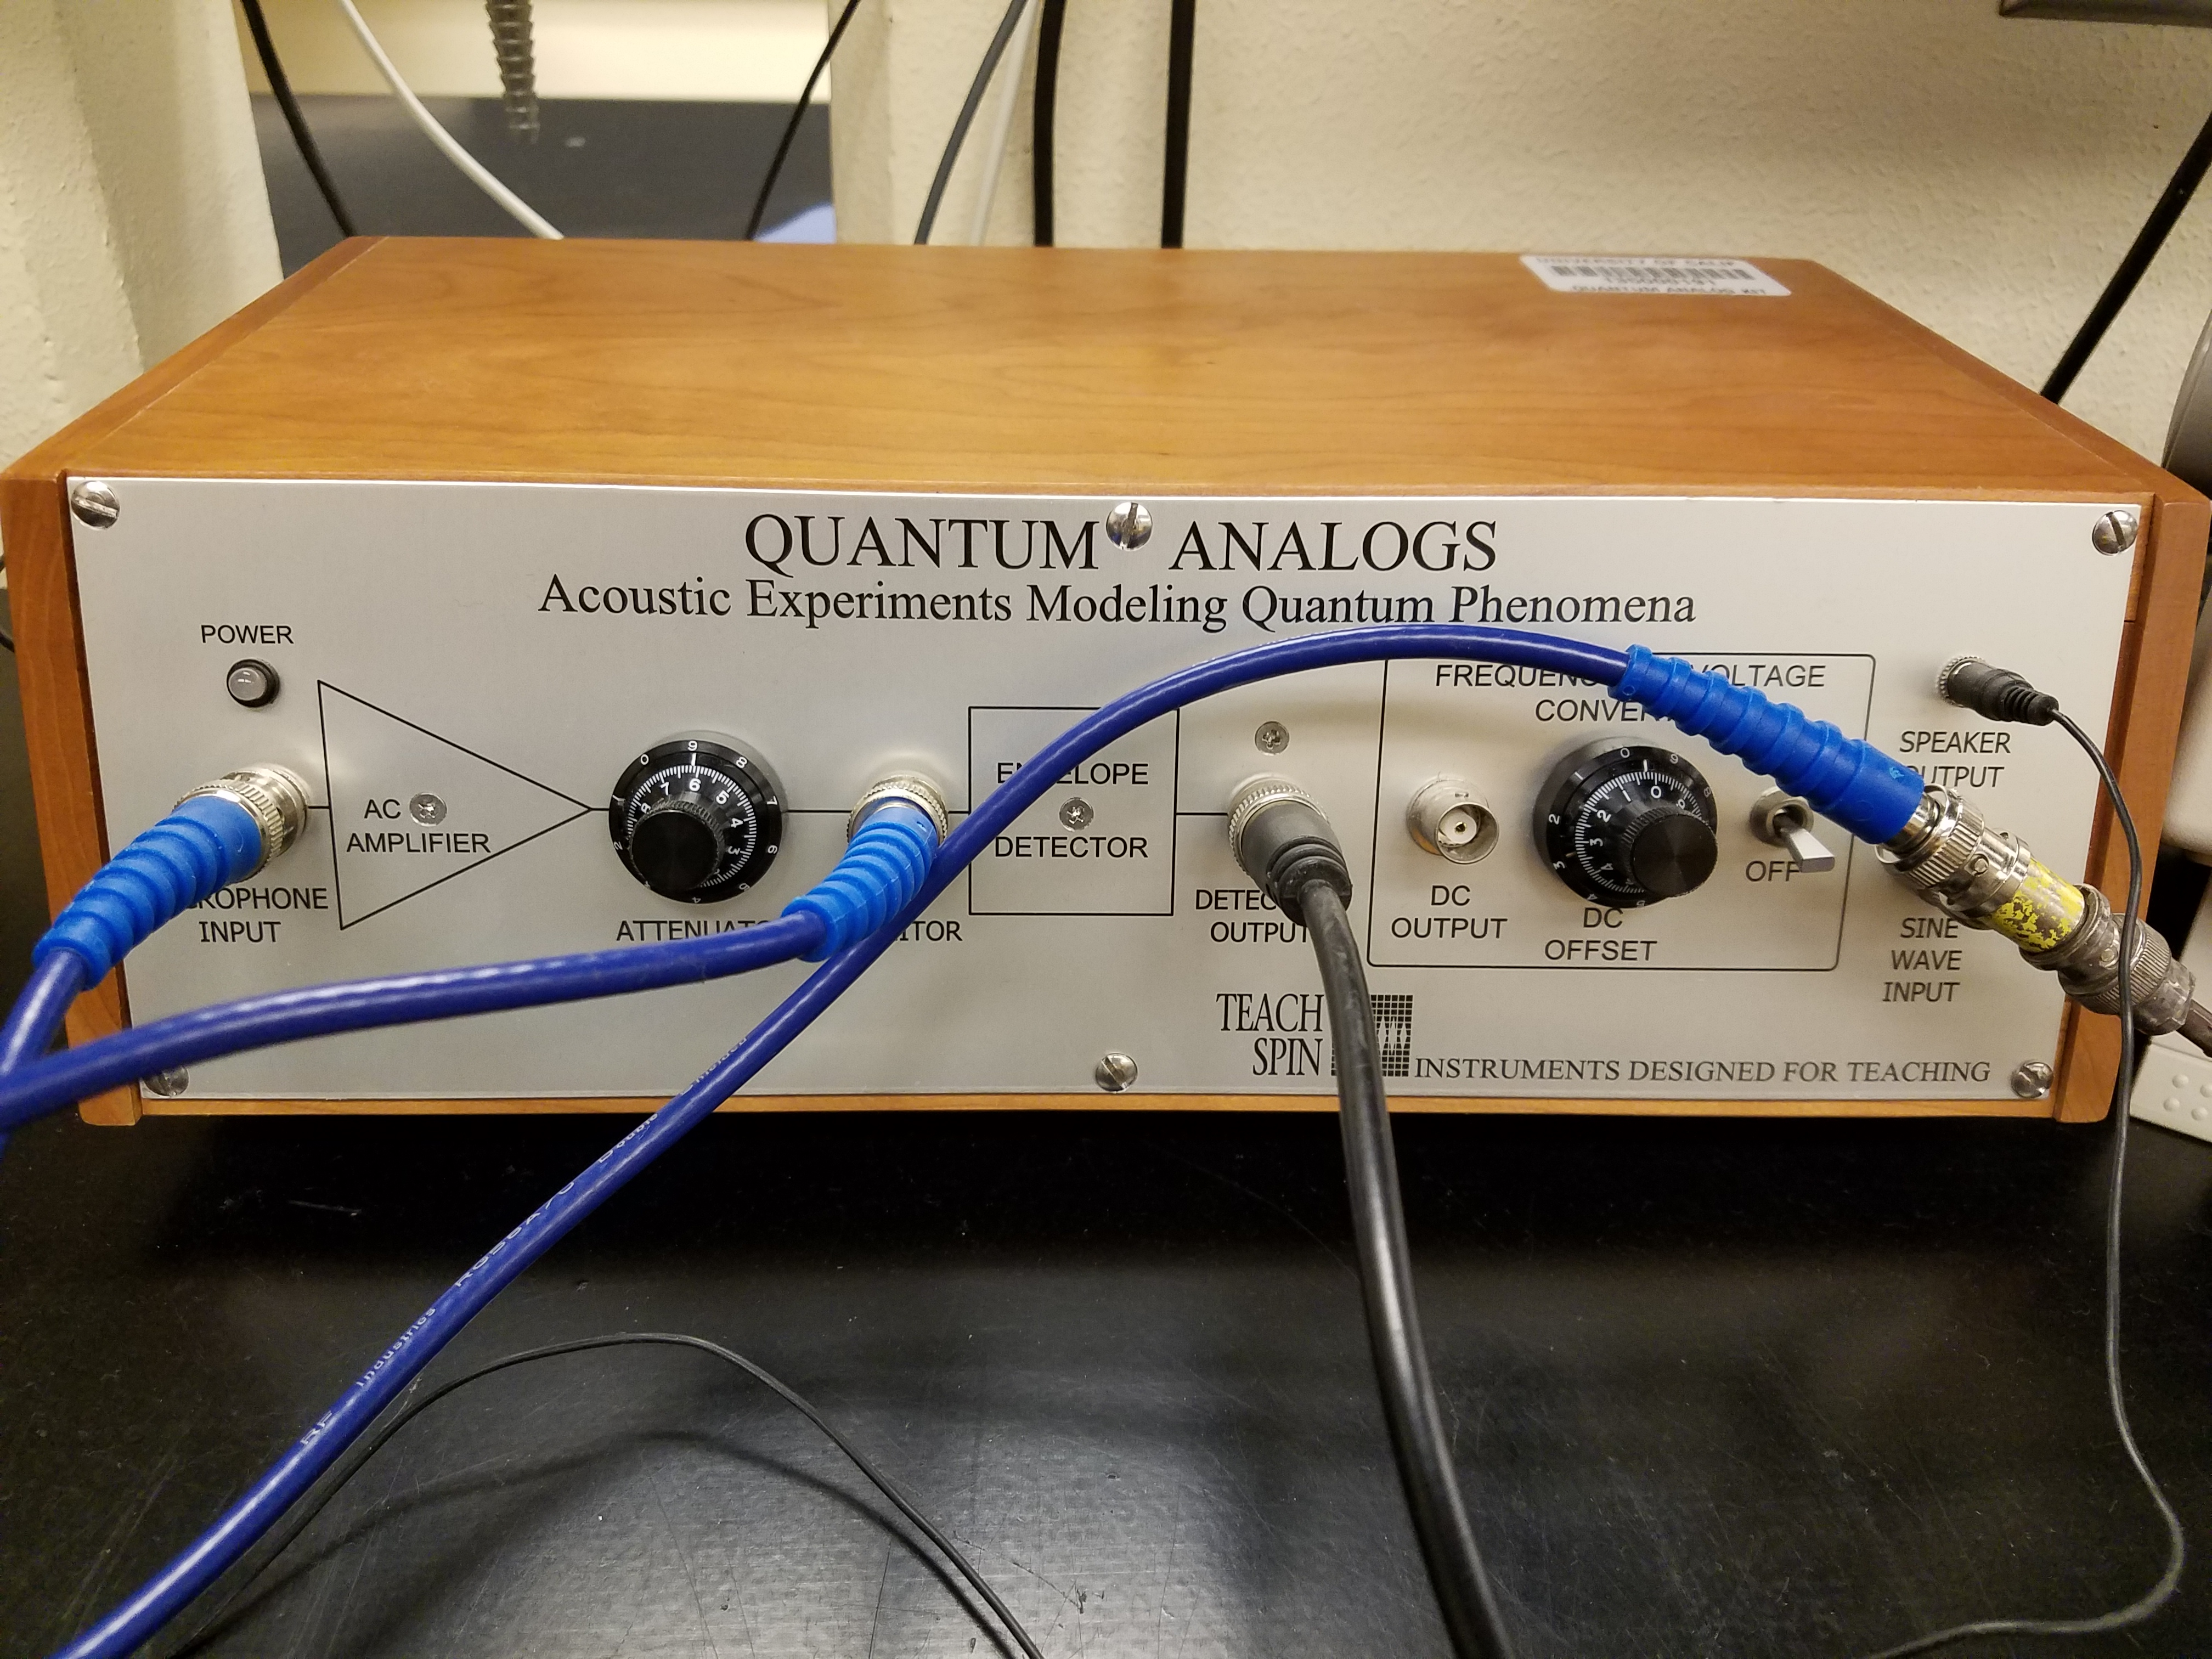
\includegraphics[scale = 0.05]{Setup/AnalogsDevice}
%		\caption{Quantum Analogs Controller}
%		\end{wrapfigure}
%
%		\begin{wrapfigure}{r}{0.5\textwidth}
%		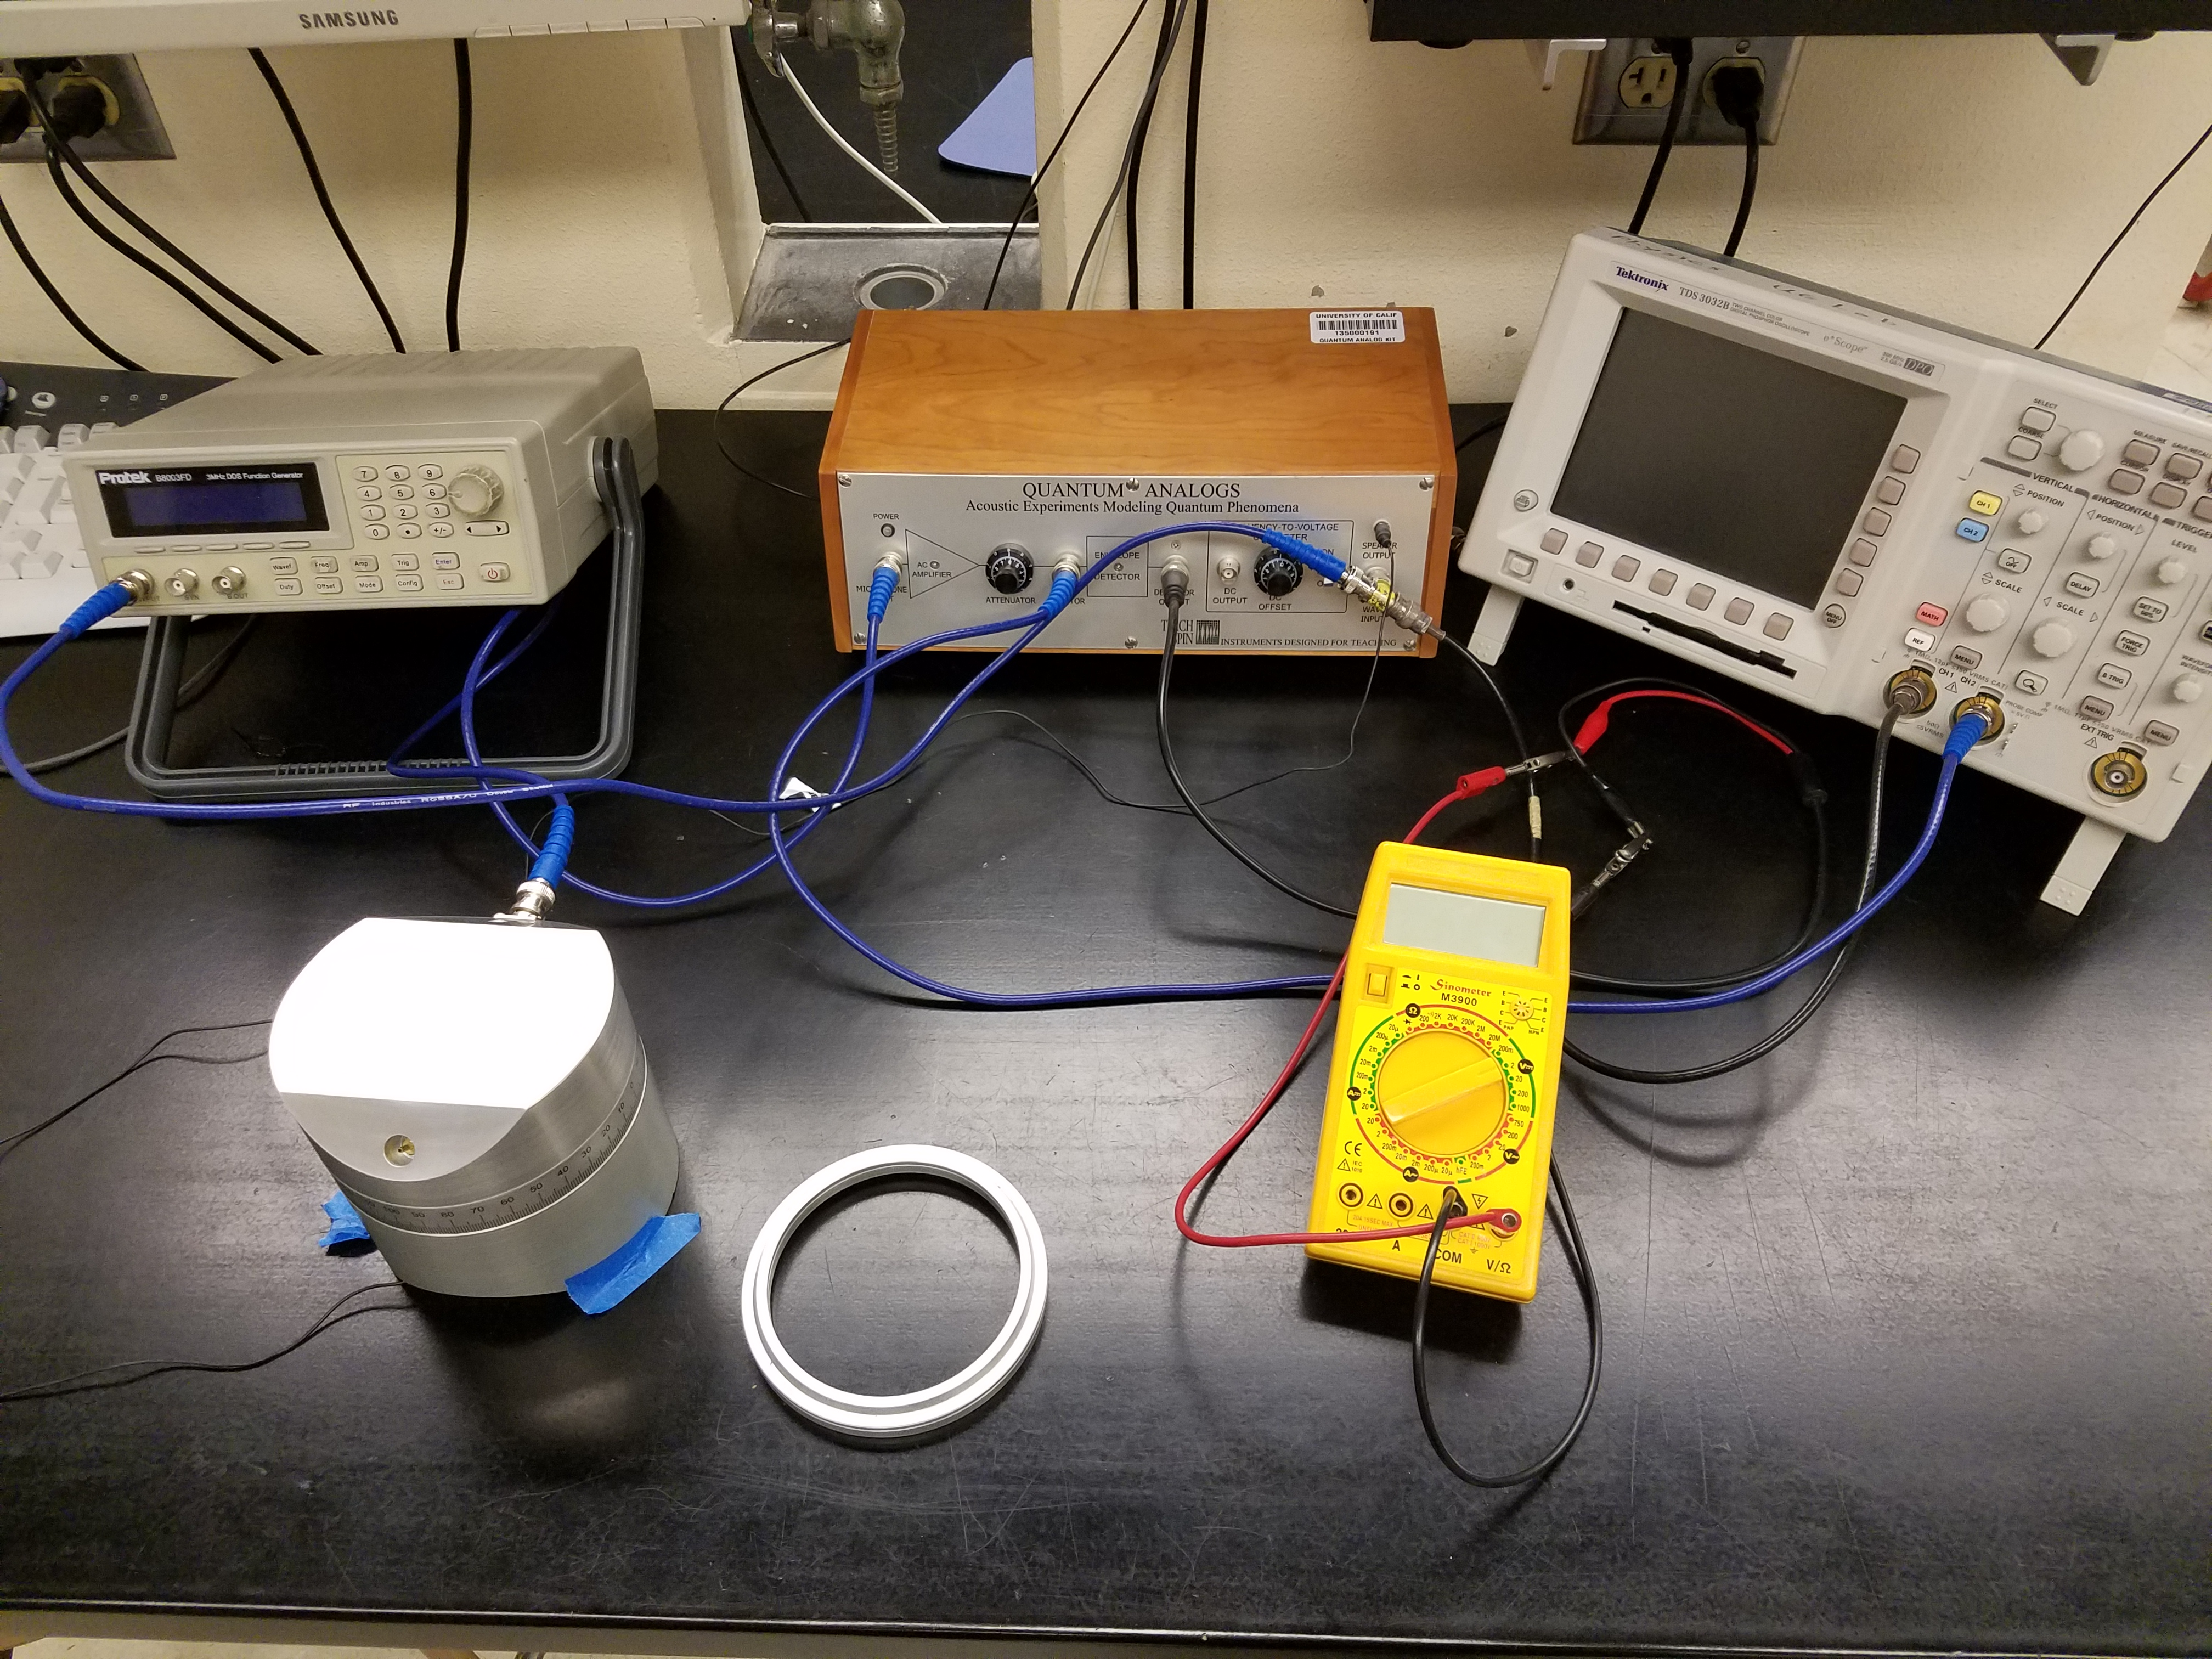
\includegraphics[scale = 0.05]{Setup/Table}
%		\caption{Quantum Analogs Controller}
%		\end{wrapfigure}

		\begin{figure}[H]
			\captionsetup{justification = centering}
			\centering
			\subfloat[Quantum Analogs Controller]{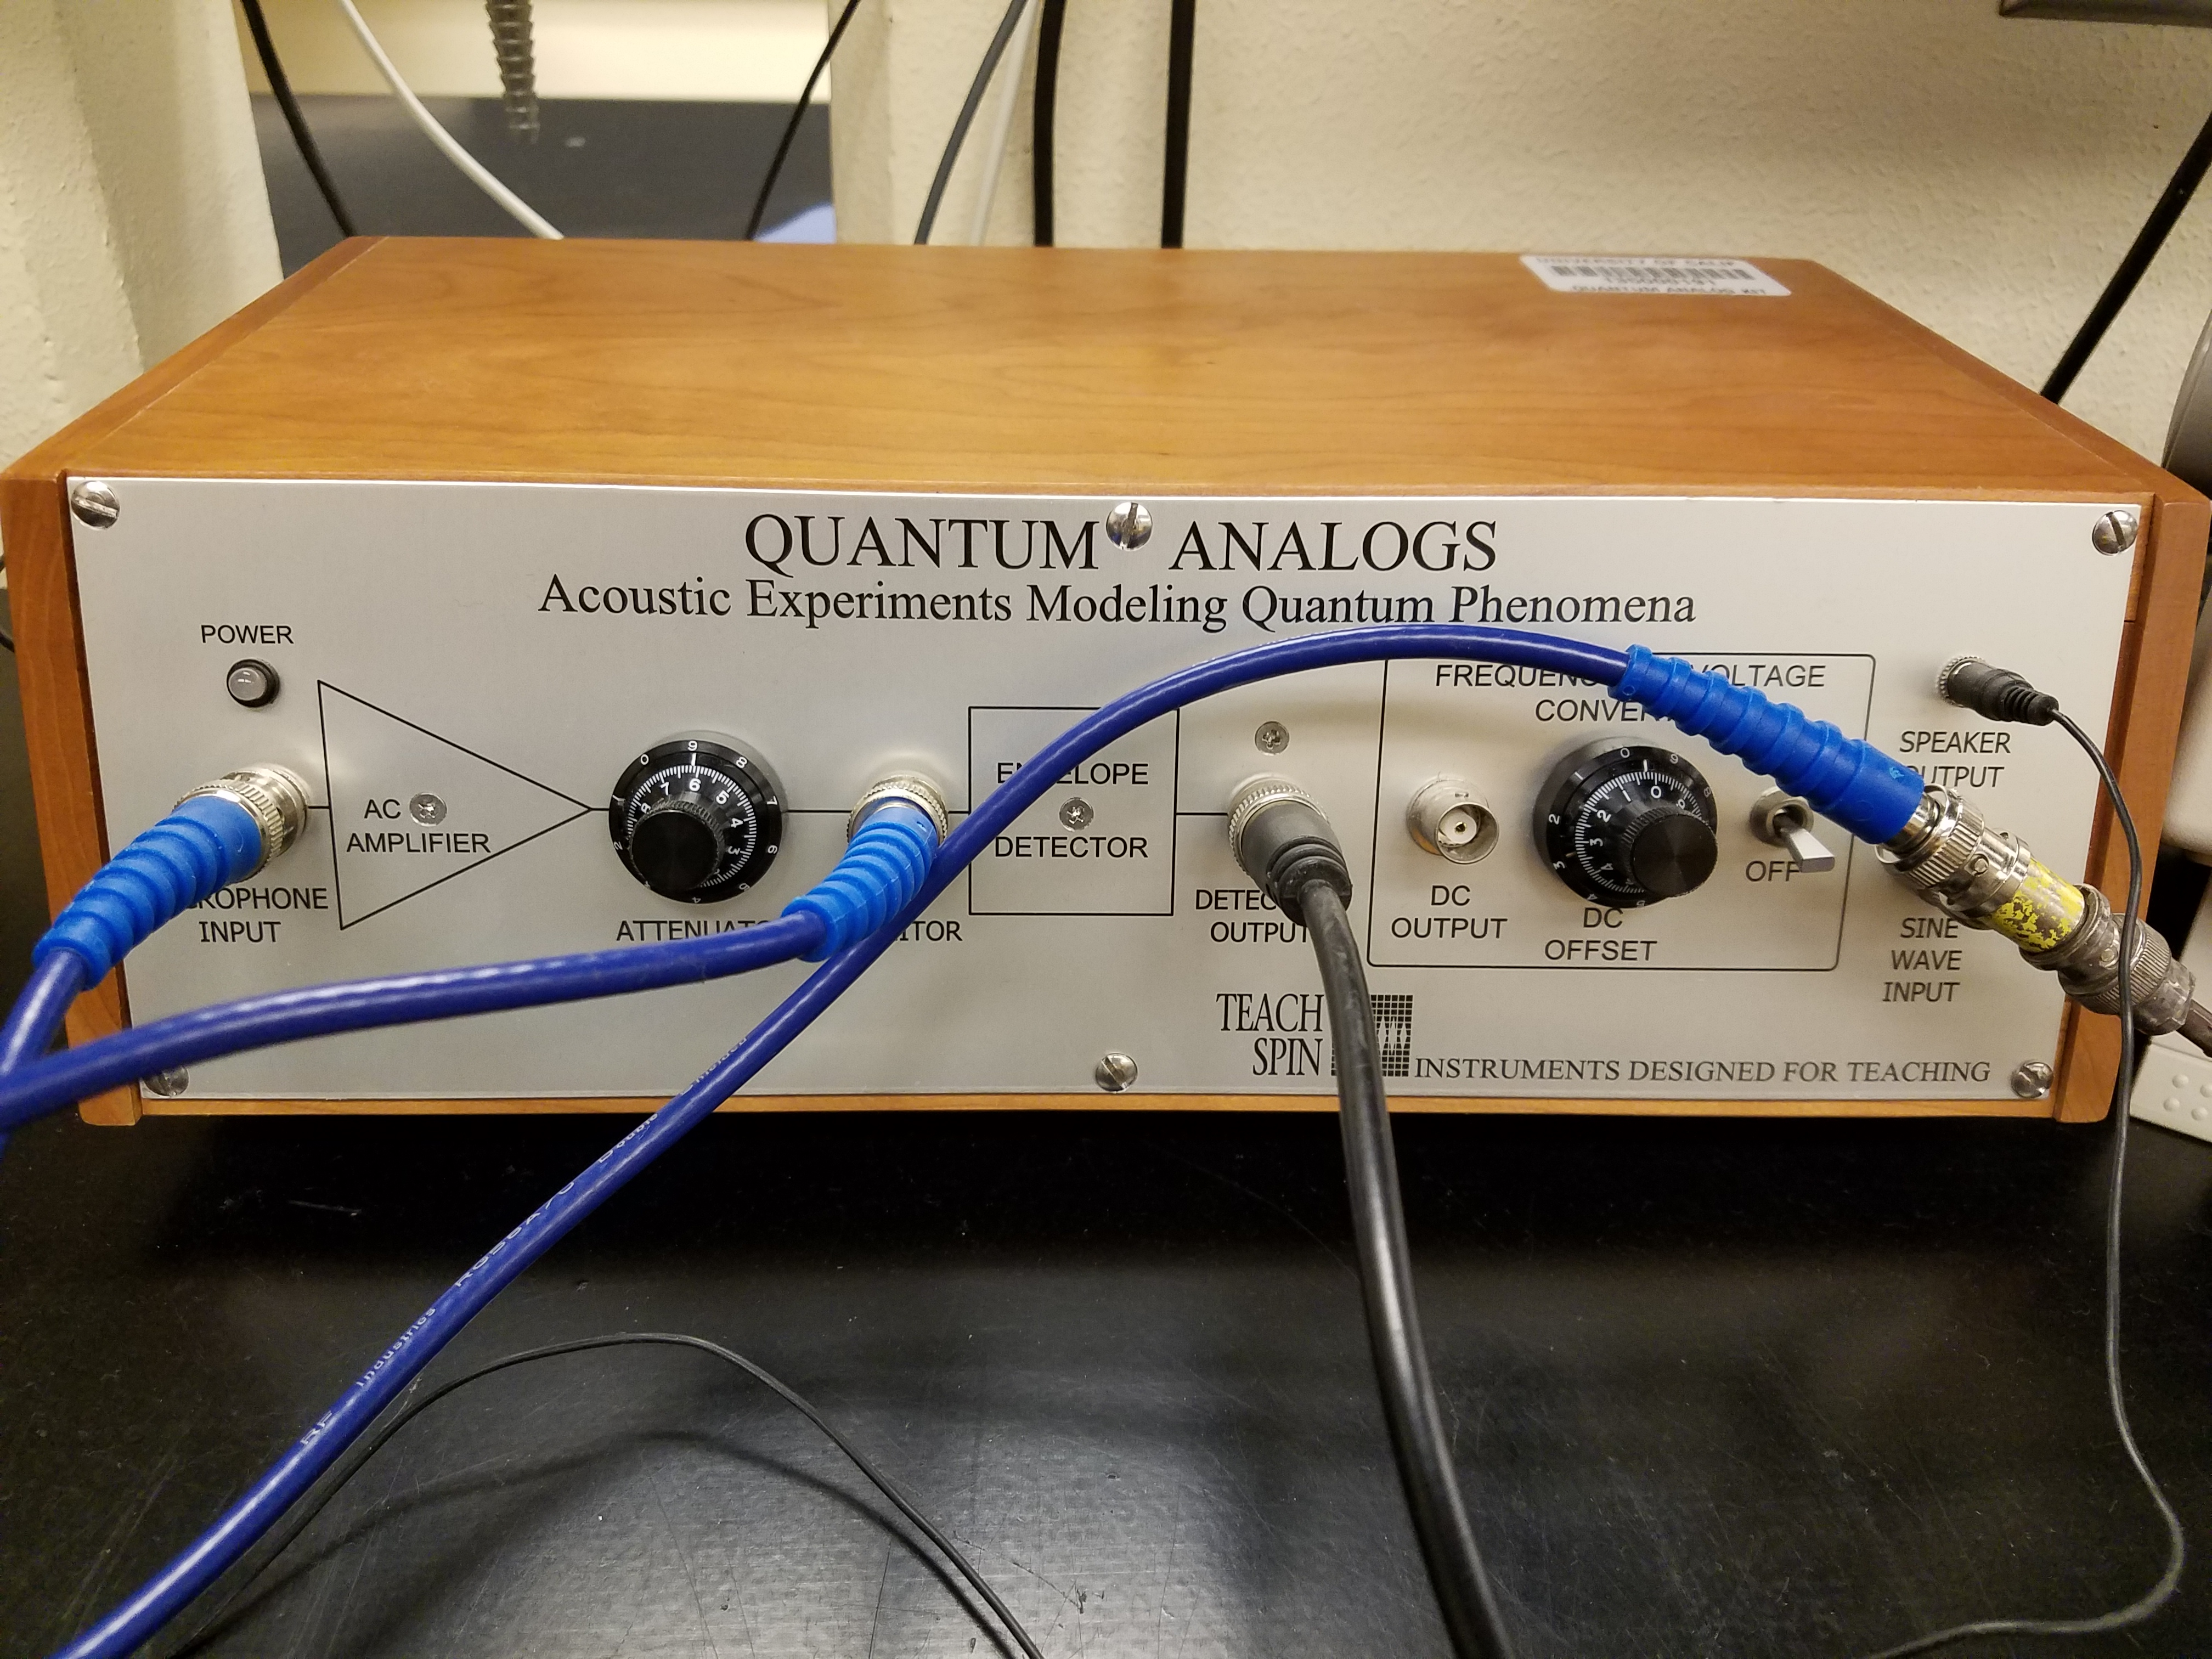
\includegraphics[width=0.4\textwidth]{Setup/AnalogsDevice}\label{QAController}}
			\qquad
			\subfloat[Lab bench]{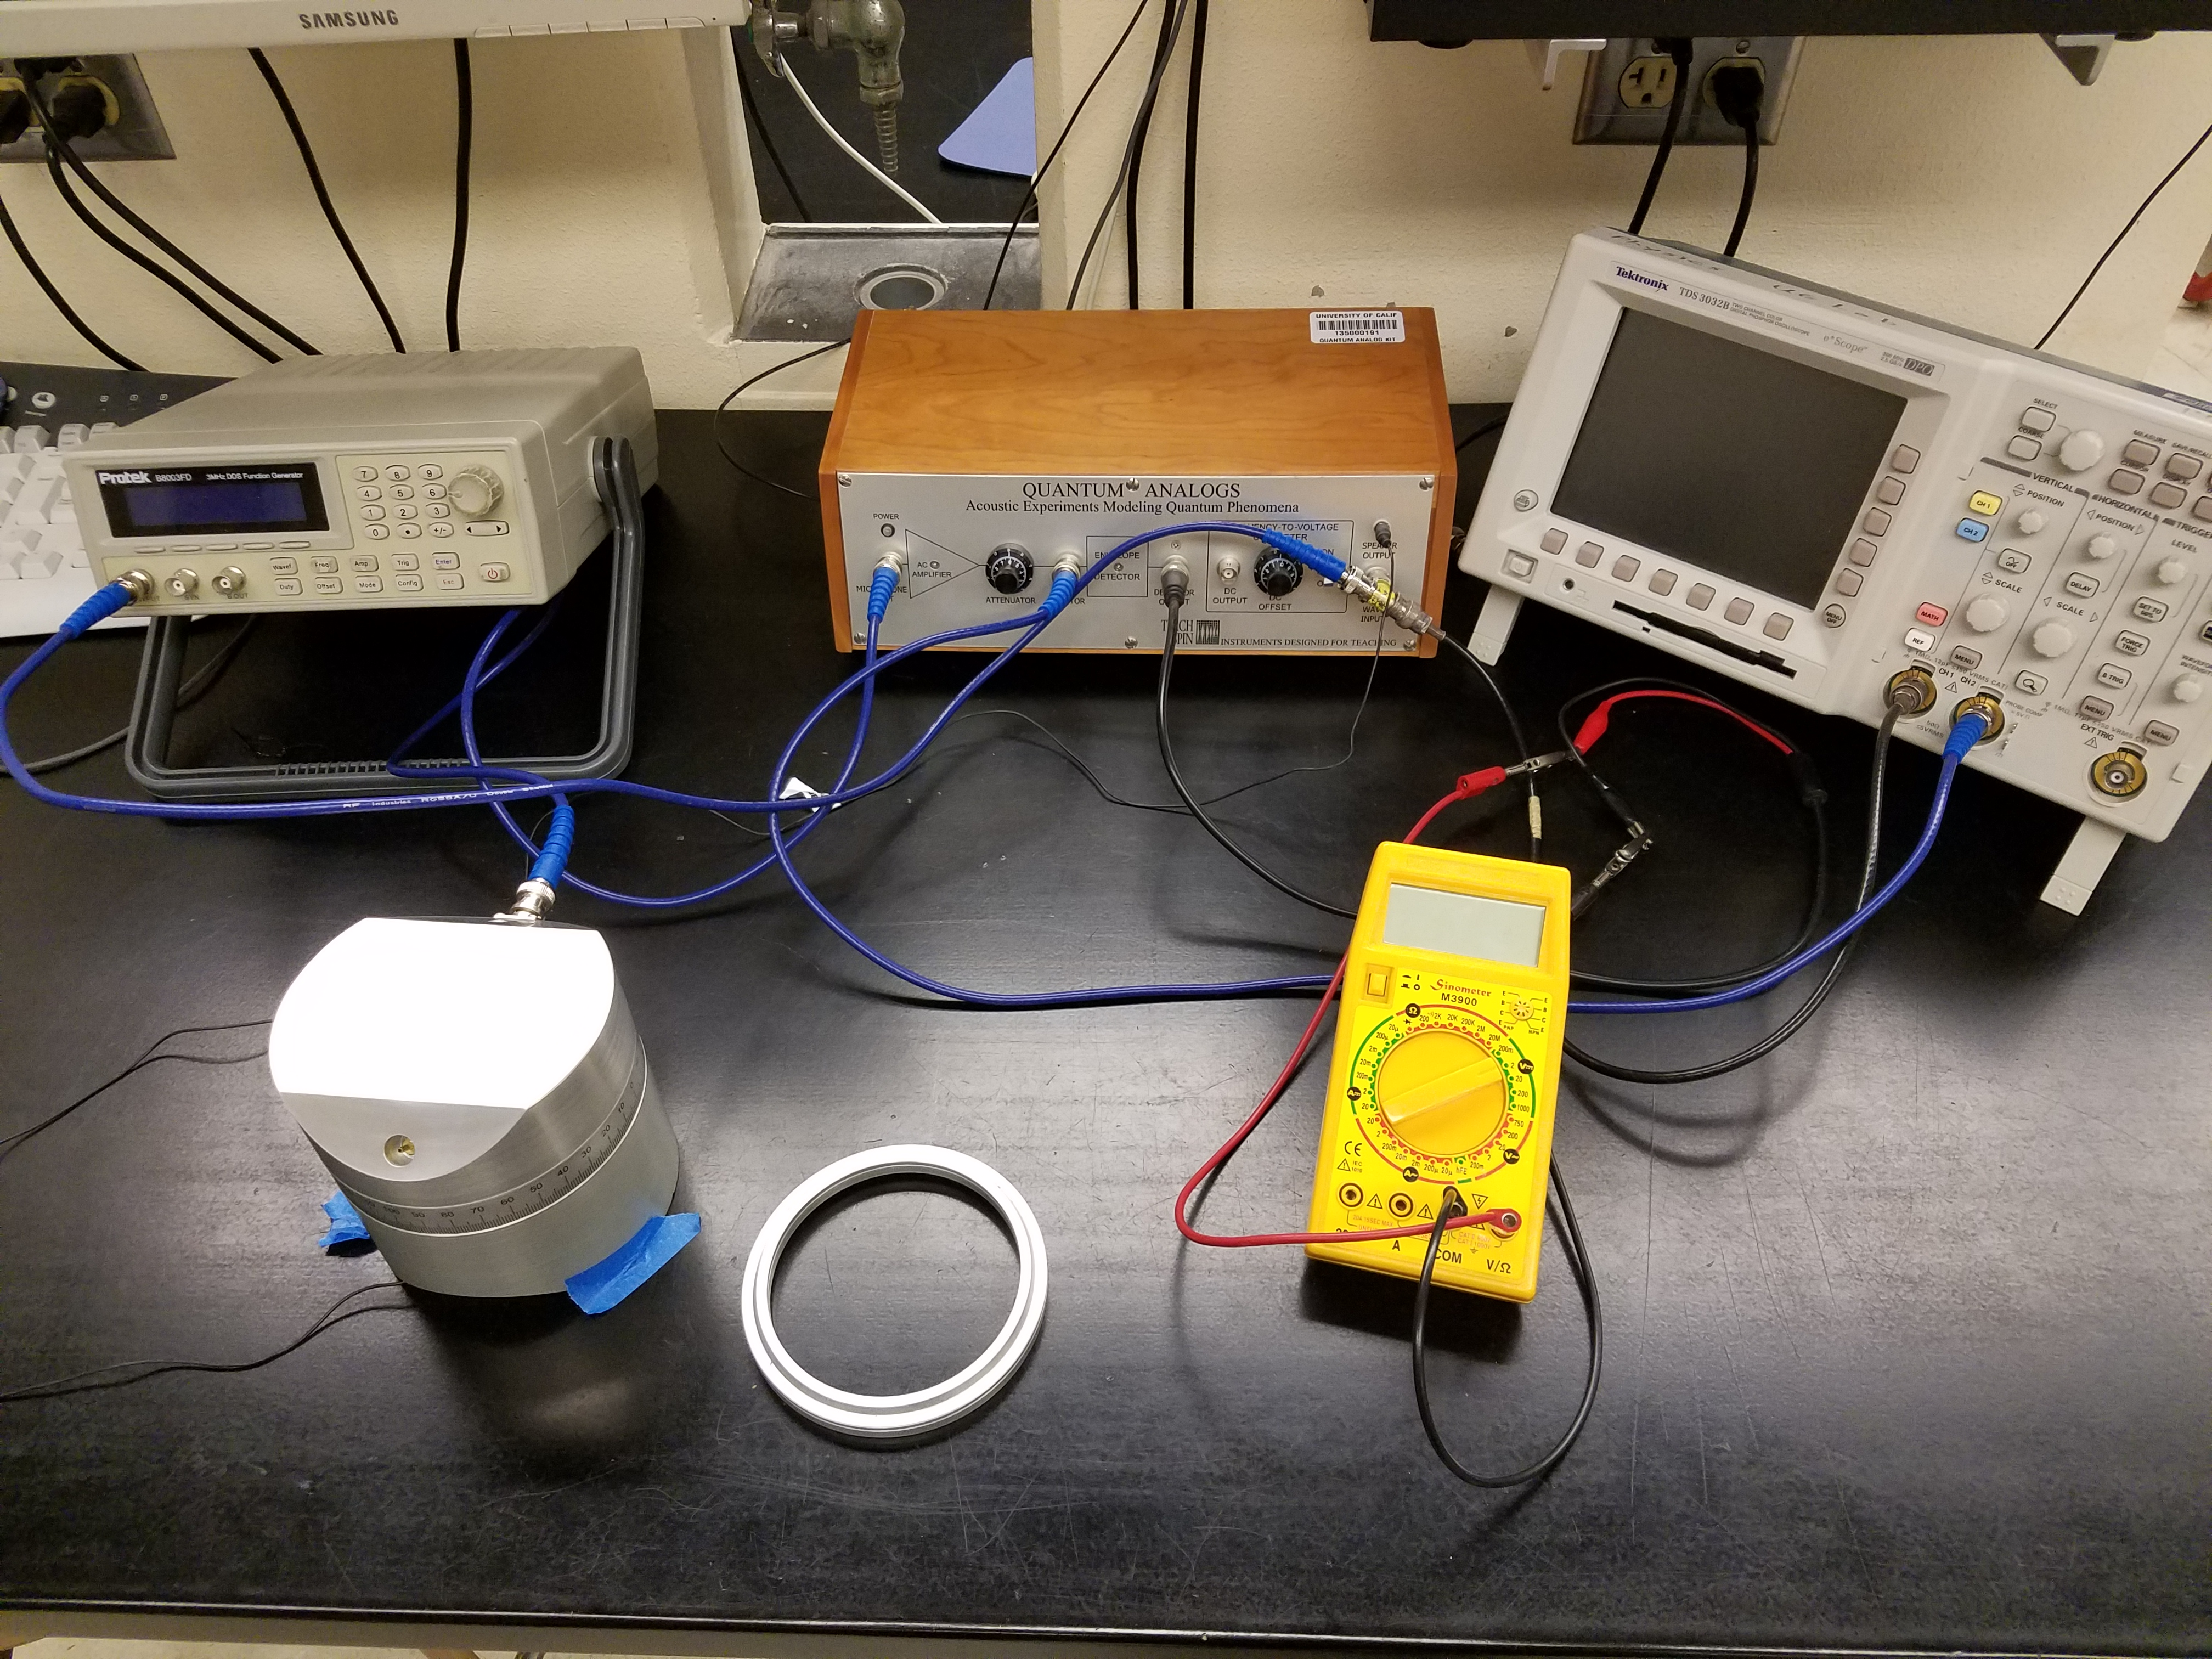
\includegraphics[width=0.4\textwidth]{Setup/Table}
			\label{Setup}}
			\caption{The \emph{Quantum Analogs Controller} \protect\subref{QAController} and our table setup up \protect\subref{Setup}}
			\label{experiment}
		\end{figure}

%		\subsection{Acoustic Resonances of the Spherical Cavity}
		
		\subsection{Frequency Spectrum}
		Before we begin mapping out resonant frequencies, we need to find the frequency range where the cavity response is linear. To do this, we set the attenuation to maximum (10), $\alpha = 180 \deg$, and sweep the frequency from $1$ Hz to $\approx 8$ kHz in increments of $10$ Hz. The linear regime of the signal ranges from about $2$ kHz to $8$ kHz and is seen in \figref{LinRegime}. We use $10$ Hz increments simply to find the neighborhood of a resonance, as greater resolution is not required. After we found the linear regime, we lowered the attenuation to half (5.0) and obtained the spectrum of frequencies with clear resonances, see \figref{Raw50a180}. The two smaller peaks at $\approx 6.5$ kHz and $8$ kHz are products of cross talk, and thus not resonances.
		
		Once we restricted our attention to the linear regime, we began isolating the resonant frequencies using the oscilloscope. On the oscilloscope, a resonance will appear as in increase in the amplitude orders of magnitude larger than the characteristic scale of the signal. Near a resonance, we fine tune the frequency in increments of $1$ Hz until the amplitude is maximized. It is important to note that denominations smaller than $1$ Hz are not discernible on the oscilloscope due to the limited resolution of the screen. A table summarizing the resonant frequencies may be found in \figref{freqTable}.
		
		\begin{figure}[H]
			\captionsetup{justification = justified}
			\centering
			\subfloat[Linear regime frequency spectrum with maximum attenuation]
			{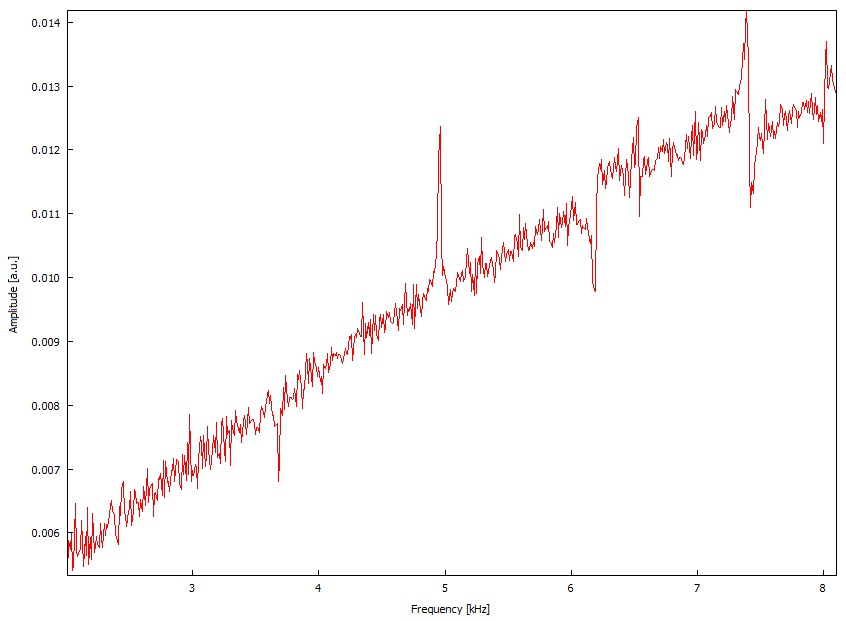
\includegraphics[width=0.4\textwidth]{2.3.2/Raw100a180.jpg}
				\label{LinRegime}}
			\qquad
			\subfloat[Linear regime frequency spectrum with half attenuated signal]{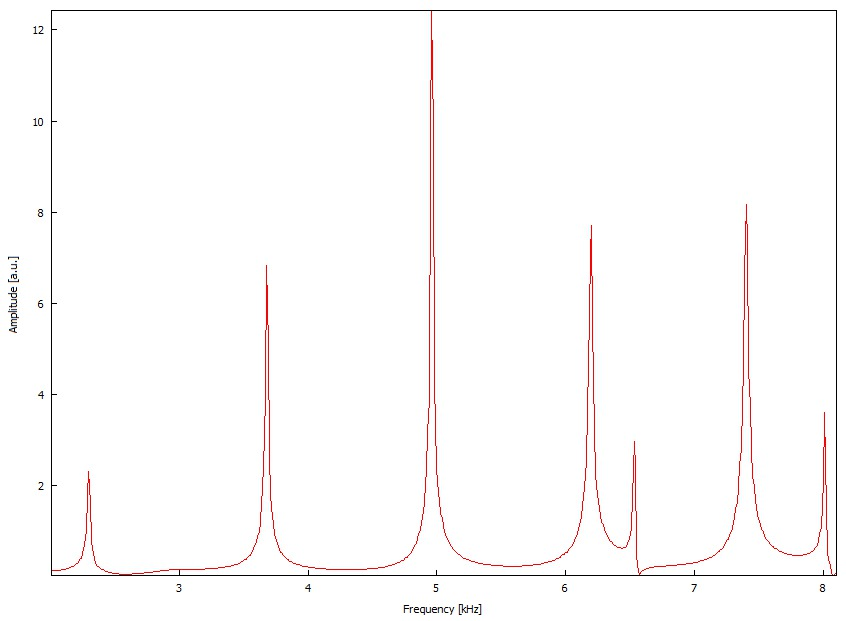
\includegraphics[width=0.4\textwidth]{2.3.2/Raw50a180.jpg}
				\label{Raw50a180}}
			\caption{Fig \protect\subref{LinRegime} shows the linear regime of the frequency spectrum with maximum attenuation. Fig \protect\subref{Raw50a180} shows that same frequency range with a half-attenuated signal.}
			\label{freqSpec}
		\end{figure}
		
		
		
		
		\subsection{Measuring Spherical Cavity Resonances with the Computer}
		In this section, we used the sound card in the computer to both generate and measure the resonances within the cavity. We set the attenuator to its highest value ($10$) to protect the sound card. The sound card output is connected to the Quantum Analogs \emph{Sine Wave Input} and to channel 1 of the oscilloscope. The \emph{AC Monitor} from the Quantum Analogs device is connected to the microphone input on the sound card and to channel 2 of the oscilloscope. 
		
		Since the equation we are modeling is a linear differential equation, we measure the frequency spectrum over the entire frequency range, with the attenuation on the Quantum Analogs device set to its maximum setting, and focus our attention to the region where the spectrum increases linearly. We determine the linear regime of frequency response is between $2$ kHz to $8.1$ kHz. The linear regime of the frequency spectrum is shown in \figref{LinRegime} in Appendix A. The large spikes indicate resonant frequencies. Once we determine the linear regime of the signal, we fine tune the attenuation and speaker amplitude to maximize signal and minimize cross-talk. The frequency spectrum for $\alpha = 180\deg$ and $50\%$ attenuation can be seen in \figref{Raw50a180} in appendix A.
		
		Starting with $\alpha = 180 \deg$ and a step size of $10$ Hz, we sweep from $2$ to $8.1$ kHz and record the amplitude. We repeat this process for $\alpha = 40\deg, 20\deg$ and $0\deg$. We resolved the peak around $5$ kHz by decreasing the step size to from $10$ Hz to $0.5$ Hz. \red{figure references} 
		
		
		
		
		
		
		
		
	\section{Results and Analysis}
		
		\subsection{Spectrum Response to varying $\alpha$}
		\red{TO DO: learn why the spectrum changes when we change alpha}
		
		Once we obtained the frequency spectrum in the linear regime of the signal, we varied $\alpha$ to observe how the spectrum changes as a function of cavity angle. 
		
		
		\begin{figure}[H]
			\centering
			\subfloat[Spectrum for $\alpha = 40\deg$]{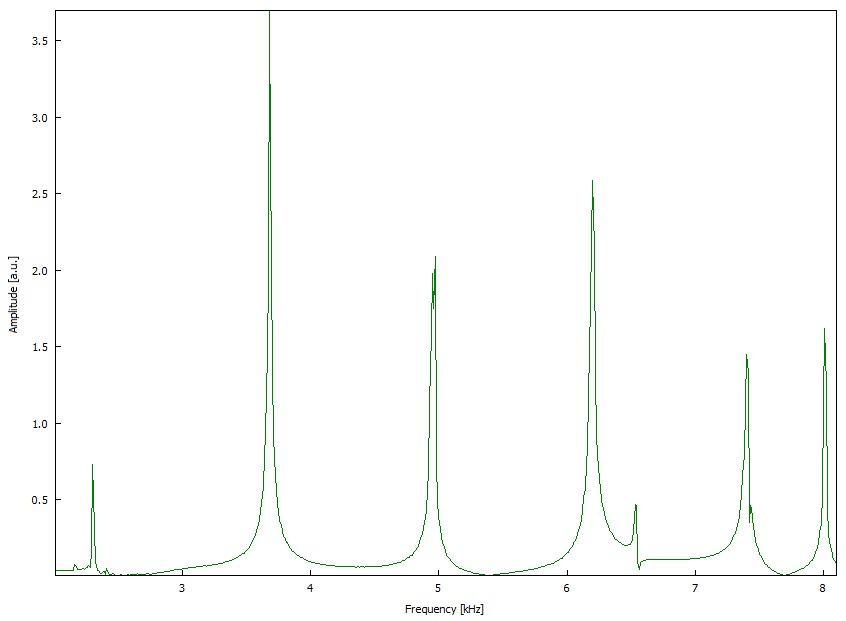
\includegraphics[width=0.3\textwidth ]{2.3.2/Raw50a40.jpg}}
			\quad
			\subfloat[Spectrum for $\alpha = 20\deg$]{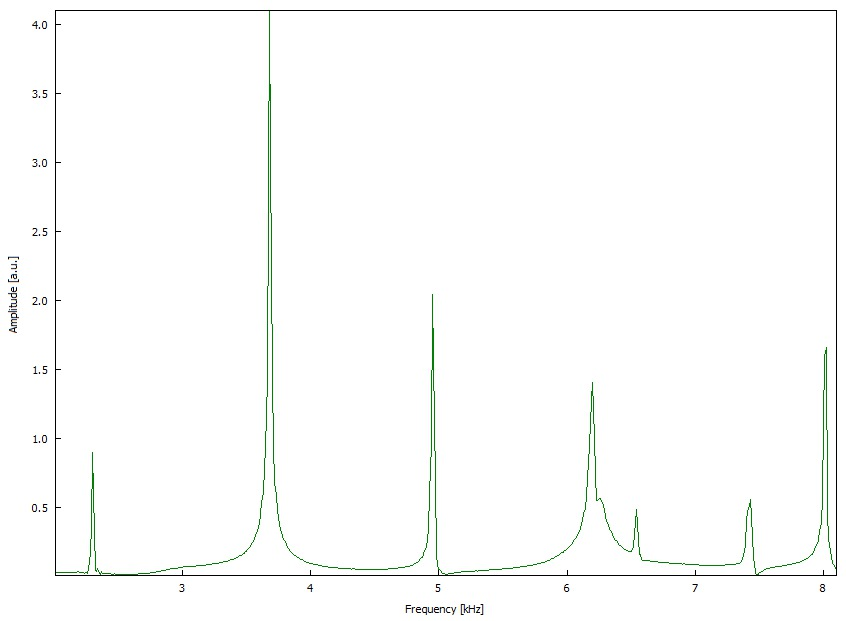
\includegraphics[width=0.3\textwidth]{2.3.2/Raw50a20.jpg}}
			\quad
			\subfloat[Spectrum for $\alpha = 0\deg$]{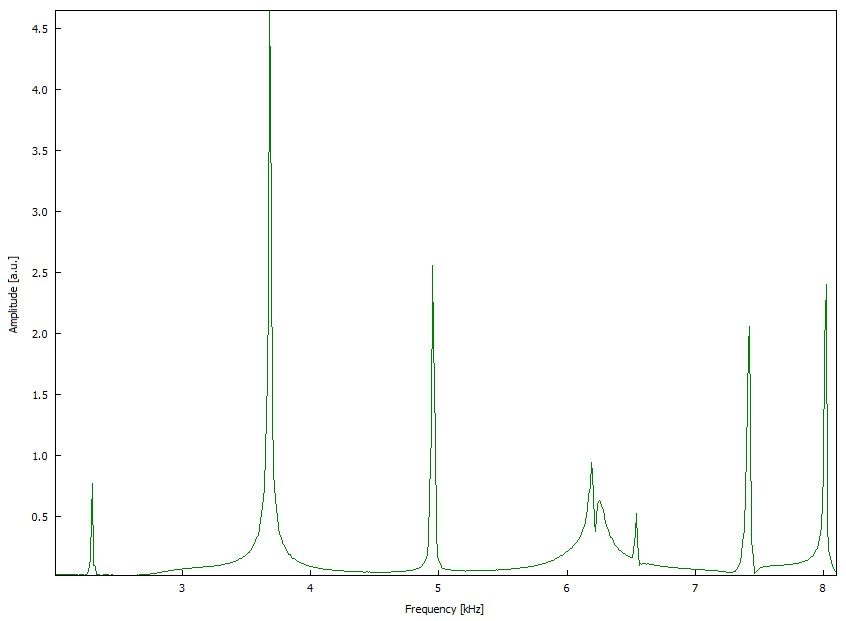
\includegraphics[width=0.3\textwidth]{2.3.2/Raw50a0.jpg}}
			\caption{Graphs showing the spectrum as we vary the cavity angle $\alpha$ from $40\deg$ to $0\deg$. We can see that as $\alpha$ decreases, the resonance at $\approx6$ kHz drops off.}
			\label{angleSpectra}
		\end{figure}
		
		\begin{figure}[H]
			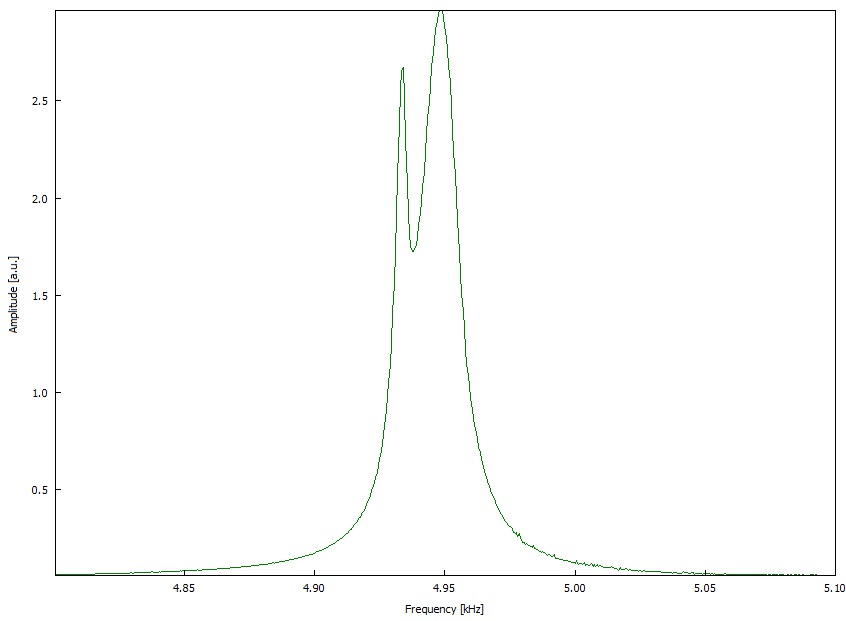
\includegraphics[width=0.3\textwidth]{2.3.2./Raw50a0res.jpg}
			\caption{Hi resolution spectrum\\ at the $5$ kHz resonance}
			\label{hiRes5K}
		\end{figure}
		
		
		\subsection{Mapping out Polar Angle Dependence at Resonance}
		\red{include attenuation value}
		Once we determined all the resonant frequencies, we began mapping out the angular dependence at each resonance. To begin, we set the angle on the cavity to $\alpha = 180 \deg$ and record the amplitude. We then decrease $\alpha$ from $180 \deg$ to $0 \deg$ in increments of $\alpha = 10\deg$. Initially, we used increments of $5\deg$ but the amplitude variation was so small, we were unable to determine if the change was due to an actual change in amplitude, or do to statistical fluctuations. 
		
		
		\begin{table}[H]
			\captionsetup{justification = centering}
			\centering
			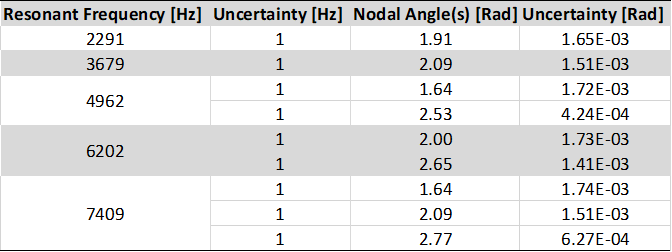
\includegraphics[width=0.7\textwidth]{Tables/ResTable.png}
			\caption{Table of measured resonant frequencies, and uncertainties, and nodal angles}
			\label{freqTable}
		\end{table}			
		
		A summary of resonant frequencies and nodal angles is shown in \cref{freqTable}. Full measurements for the amplitudes and polar angles along with uncertainties for all 5 resonant frequencies may be found in tables \cref{2291Table,3679Table,4962Table,7409Table} in Appendix A.
		
		After identifying each resonance, we mapped out the amplitude as a function of cavity angle for each resonance as seen in \figref{polarGraphs}. We may compare these to the shapes of the spherical harmonics as seen in \figref{sphereHarm} and find that each resonance corresponds to a different $\ell$ value for each spherical harmonic.
		
		\begin{figure}[H]
			\centering
			\subfloat[$\ell=1$, $m=0$ polar plot for 2291 Hz resonance]{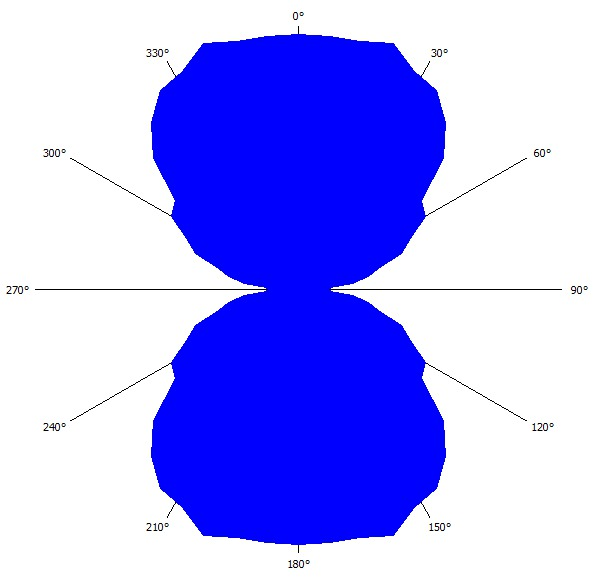
\includegraphics[width=0.4\textwidth]{2.3.2/F2291.jpg}\label{Polar2291}}
			\qquad
			\subfloat[$\ell=2$, $m=0$  plot for 3679 Hz resonance b]{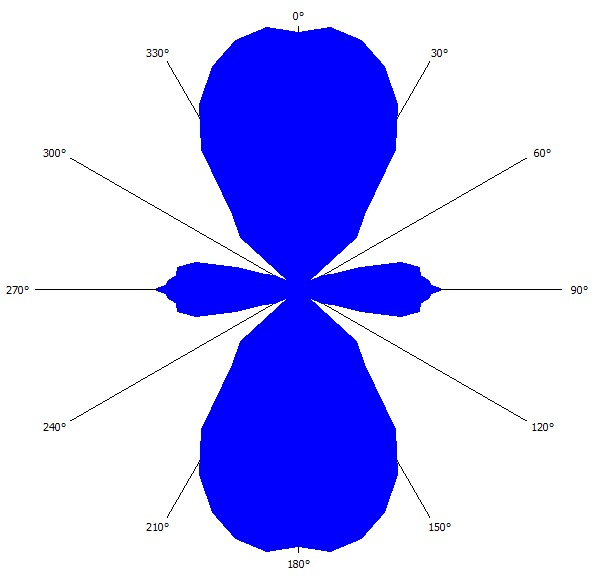
\includegraphics[width=0.4\textwidth]{2.3.2/F3679.jpg}\label{Polar3679}}
			\\
			\subfloat[$\ell=3$, $m=0$  plot for 4962 resonance]{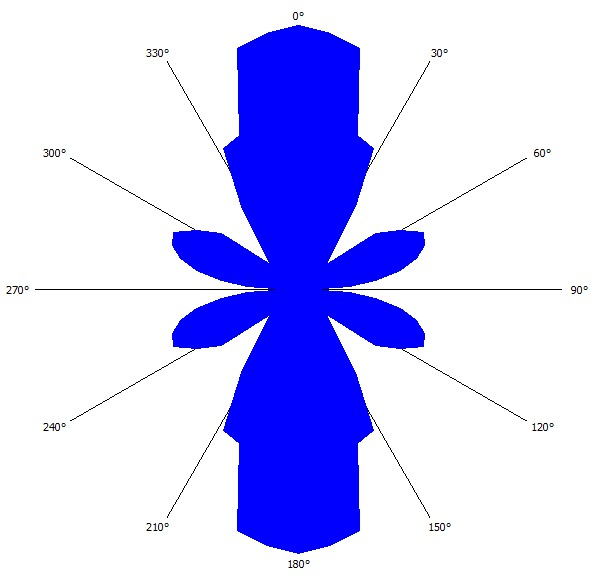
\includegraphics[width=0.4\textwidth]{2.3.2/F4962.jpg}\label{Polar4962}}
			\qquad
			\subfloat[$\ell=5$, $m=0$  plot for 7409 resonance]{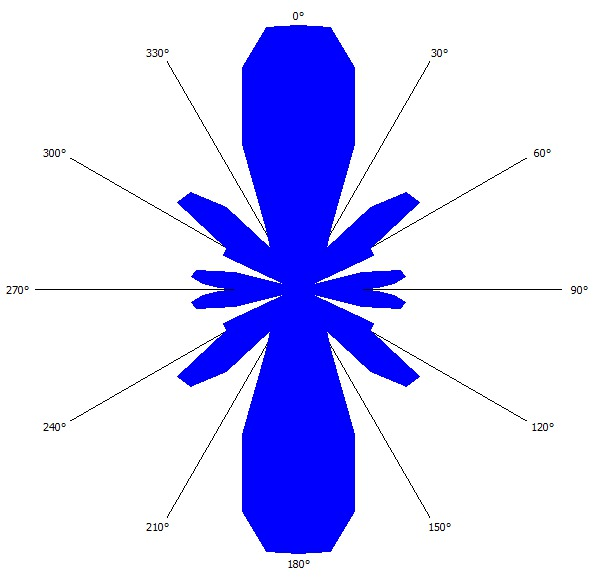
\includegraphics[width=0.4\textwidth]{2.3.2/F6202.jpg}\label{Polar6202}}
			\caption{Acoustic amplitude vs polar angle ($\theta$) with azimuthal angle $\varphi = 0$ for 4 resonant frequencies. Comparing these to the spherical harmonics in \figref{sphereHarm}, it is possible to determine the angular momentum quantum number $\ell$ for each resonance.}
			\label{polarGraphs}
		\end{figure}
	
		
		
		\subsection{$\ell=1$ Degeneracy}
		Recall that a quantum system with angular momentum $\ell$ has a $(2\ell+1)$ degeneracy of states. It is possible to resolve these degeneracies by breaking the spherical symmetry of the cavity. We achieve this by introducing the spacing rings into the cavity, simulating a magnetic field which gives a quantization axis to the system. This process is visualized in \figref{degenResolution} where we can observe the peak splitting as the spacing is increased. The lower frequency is the $m=0$ state and the higher frequency is degenerate for $m=\pm1$.
		
		
		
		\begin{figure}[H]
			\centering
			\subfloat[$\ell=1$ resnonance with spherical symmetry.]{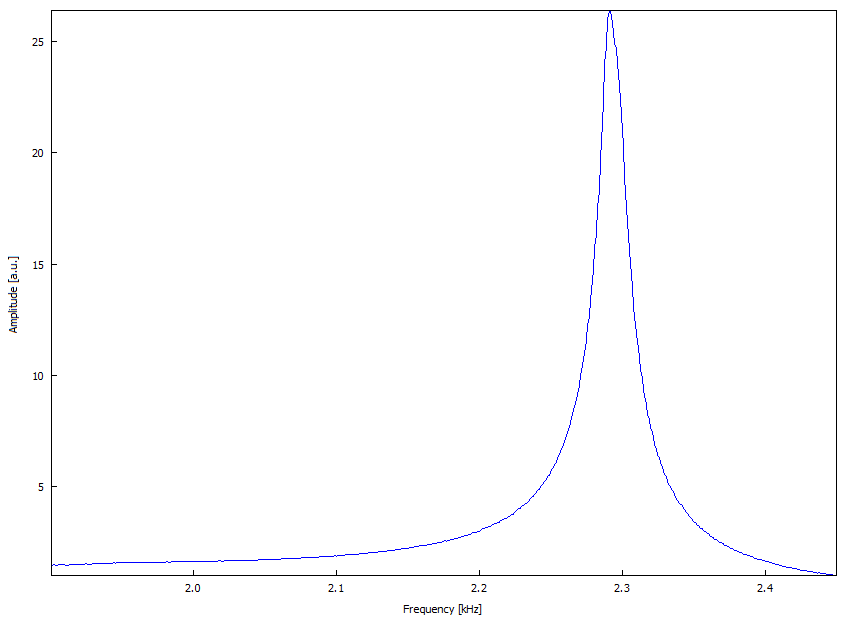
\includegraphics[width=0.45\textwidth]{Day4/L1ResonanceSpectrum.png}\label{degenResolutionSphere}}
			\quad
			\subfloat[$\ell=1$ resnonance with $3$ mm spacing.]{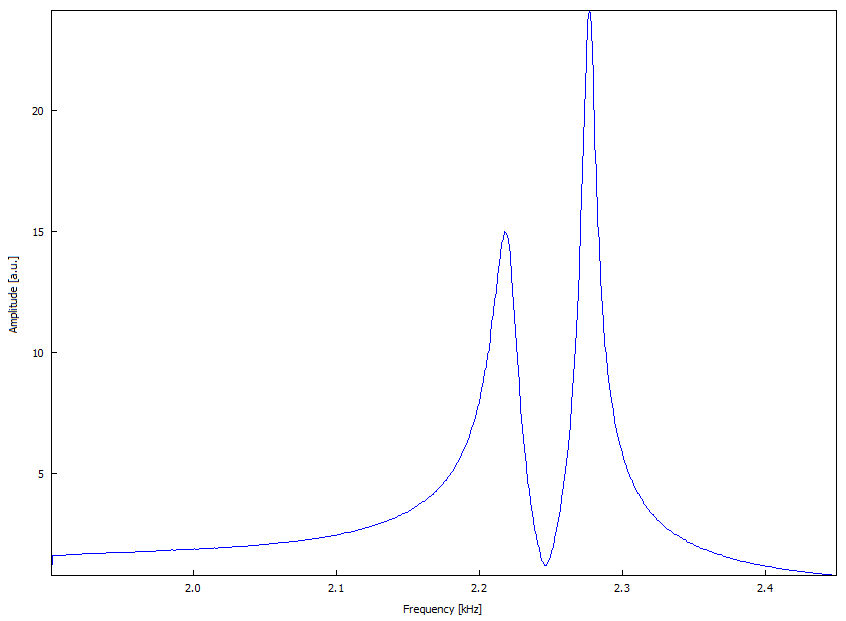
\includegraphics[width=0.45\textwidth]{Day4/L1ResonanceSpectrum3mm.png}\label{degenResolution3mm}}
			\\
			\subfloat[$\ell=1$ resnonance with $6$ mm spacing.]{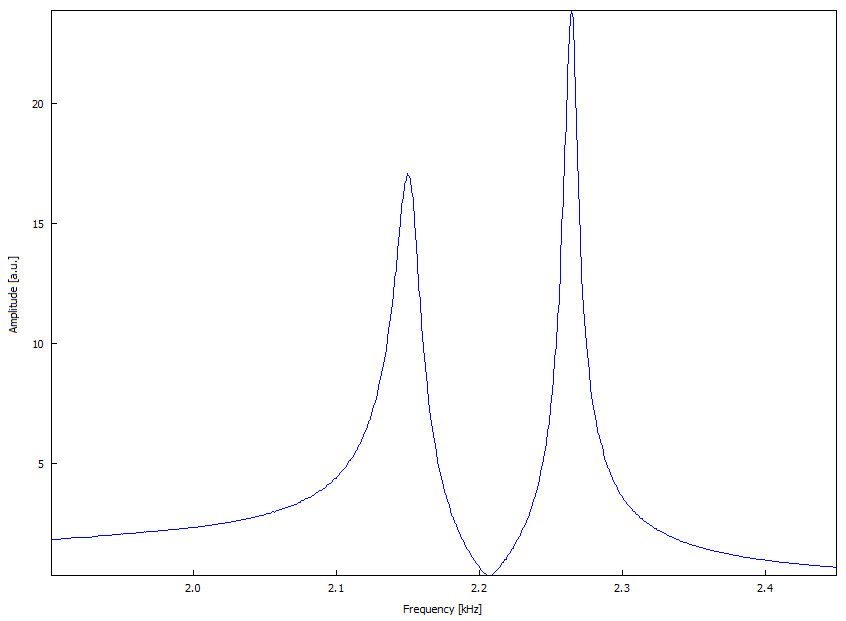
\includegraphics[width=0.45\textwidth]{Day4/L1ResonanceSpectrum6mm.png}\label{degenResolution6mm}}
			\quad
			\subfloat[$\ell=1$ resnonance with $9$ mm spacing]{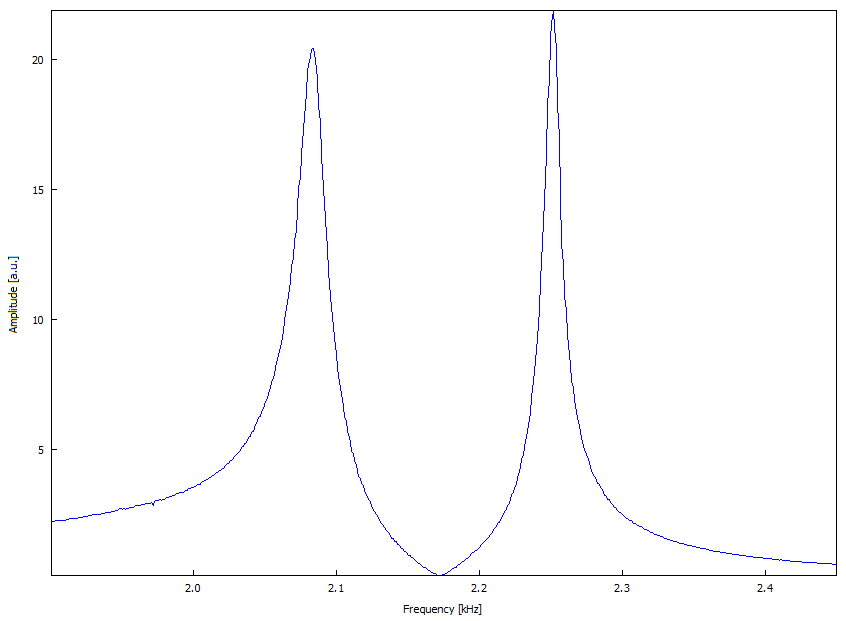
\includegraphics[width=0.45\textwidth]{Day4/L1ResonanceSpectrum9mm.png}\label{degenResolution9mm}}
			\caption{We can see as we break the spherical symmetry by introducing spacer rings to the cavity, the degeneracy in the $\ell=1$ resonance is lifted and we can resolve the $\ell = 0$ and $\ell = \pm1$ peaks.}
			\label{degenResolution}
		\end{figure}
	
	
	
		We may further investigate by examining polar plots of the amplitude to determine the magnetic quantum number $m$. \figref{9mmPolarliftedDegeneracy} shows the polar graphs of acoustic pressure vs. azimuthal angle $\varphi$ for a cavity with the maximal separation of $9$ mm. Polar amplitude graphs for the $3$ mm and $6$ mm spacing rings can be seen in \figref{3mmliftedDegeneracy} and \figref{6mmliftedDegeneracy} in the appendix.
		
		\begin{figure}[H]
			\centering
			\subfloat[$\ell=1$, $m=0$ orbital with 9mm spacing.]{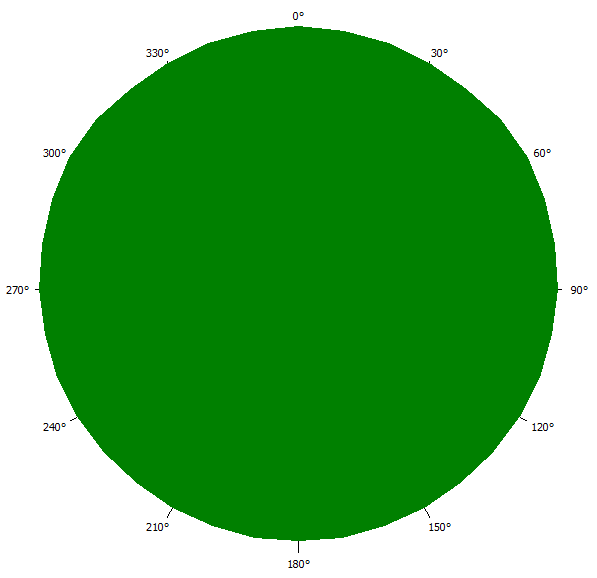
\includegraphics[width=0.4\textwidth]{Day4/L19mmPolar2084_806.png}\label{liftedDegeneracyL1M0}}
			\qquad
			\subfloat[$\ell=1$, $m=\pm1$ orbital with 9mm spacing.]{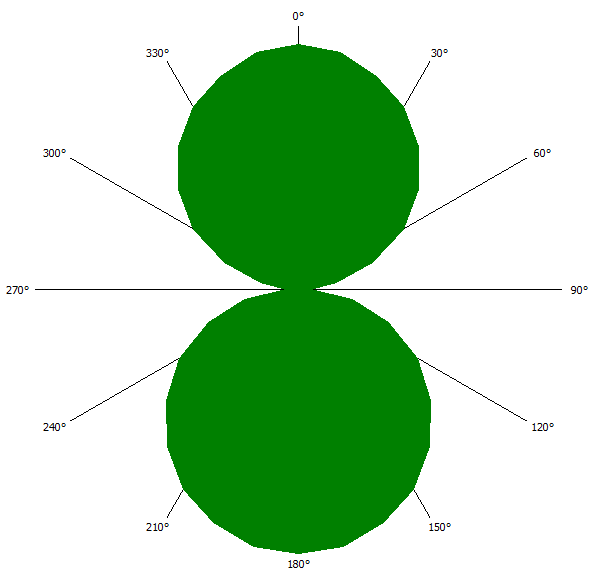
\includegraphics[width=0.4\textwidth]{Day4/L19mmPolar2251_140.png}\label{liftedDegeneracyL1M1}}			
%		\caption{Acoustic amplitude vs azimuthal angle $(\varphi)$ for polar angle $(\theta=0)$ cavity with broken symmetry. We can see that the degeneracy for the $\ell=1$ resonance is partially lifted. The $m=\pm1$ states are still degenerate since they are symmetric with respect to the azimuthal angle phi.}
			\caption{Projections of acoustic amplitude vs azimuthal angle $(\varphi)$ onto the $\theta=0$ plane. Angle markings indicate the azimuthal angle $\varphi$. We can see that the degeneracy for the $\ell=1$ resonance is partially lifted. The $m=\pm1$ states are still degenerate since they are symmetric with respect to the azimuthal angle $\varphi$.}
			\label{9mmPolarliftedDegeneracy}		
		\end{figure}

	The two states $m=\pm1$ are degenerate because they are symmetric under rotations to the azimuthal angle $\varphi$. This can be seen in the $\varphi=0$ projections of the spherical harmonics in \figref{L1M1Comparison}. The $\varphi=0$ projection of $\Ylm{1}{0}$, as seen in \figref{sphHarml1m0}, is exactly the shape of the orbital we measured in \figref{liftedDegeneracyL1M0}. Similarly, the shape of the $\varphi=0$ projection of $\Ylm{1}{1}$ in \figref{sphHarml1m1} is symmetric in $\varphi$ and matches the $\theta=0$ projection of \figref{liftedDegeneracyL1M1}.
	
	\begin{figure}[H]
		\centering
		\subfloat[Projection of $\Ylm{1}{0}$ onto the $\varphi = 0$ plane.]{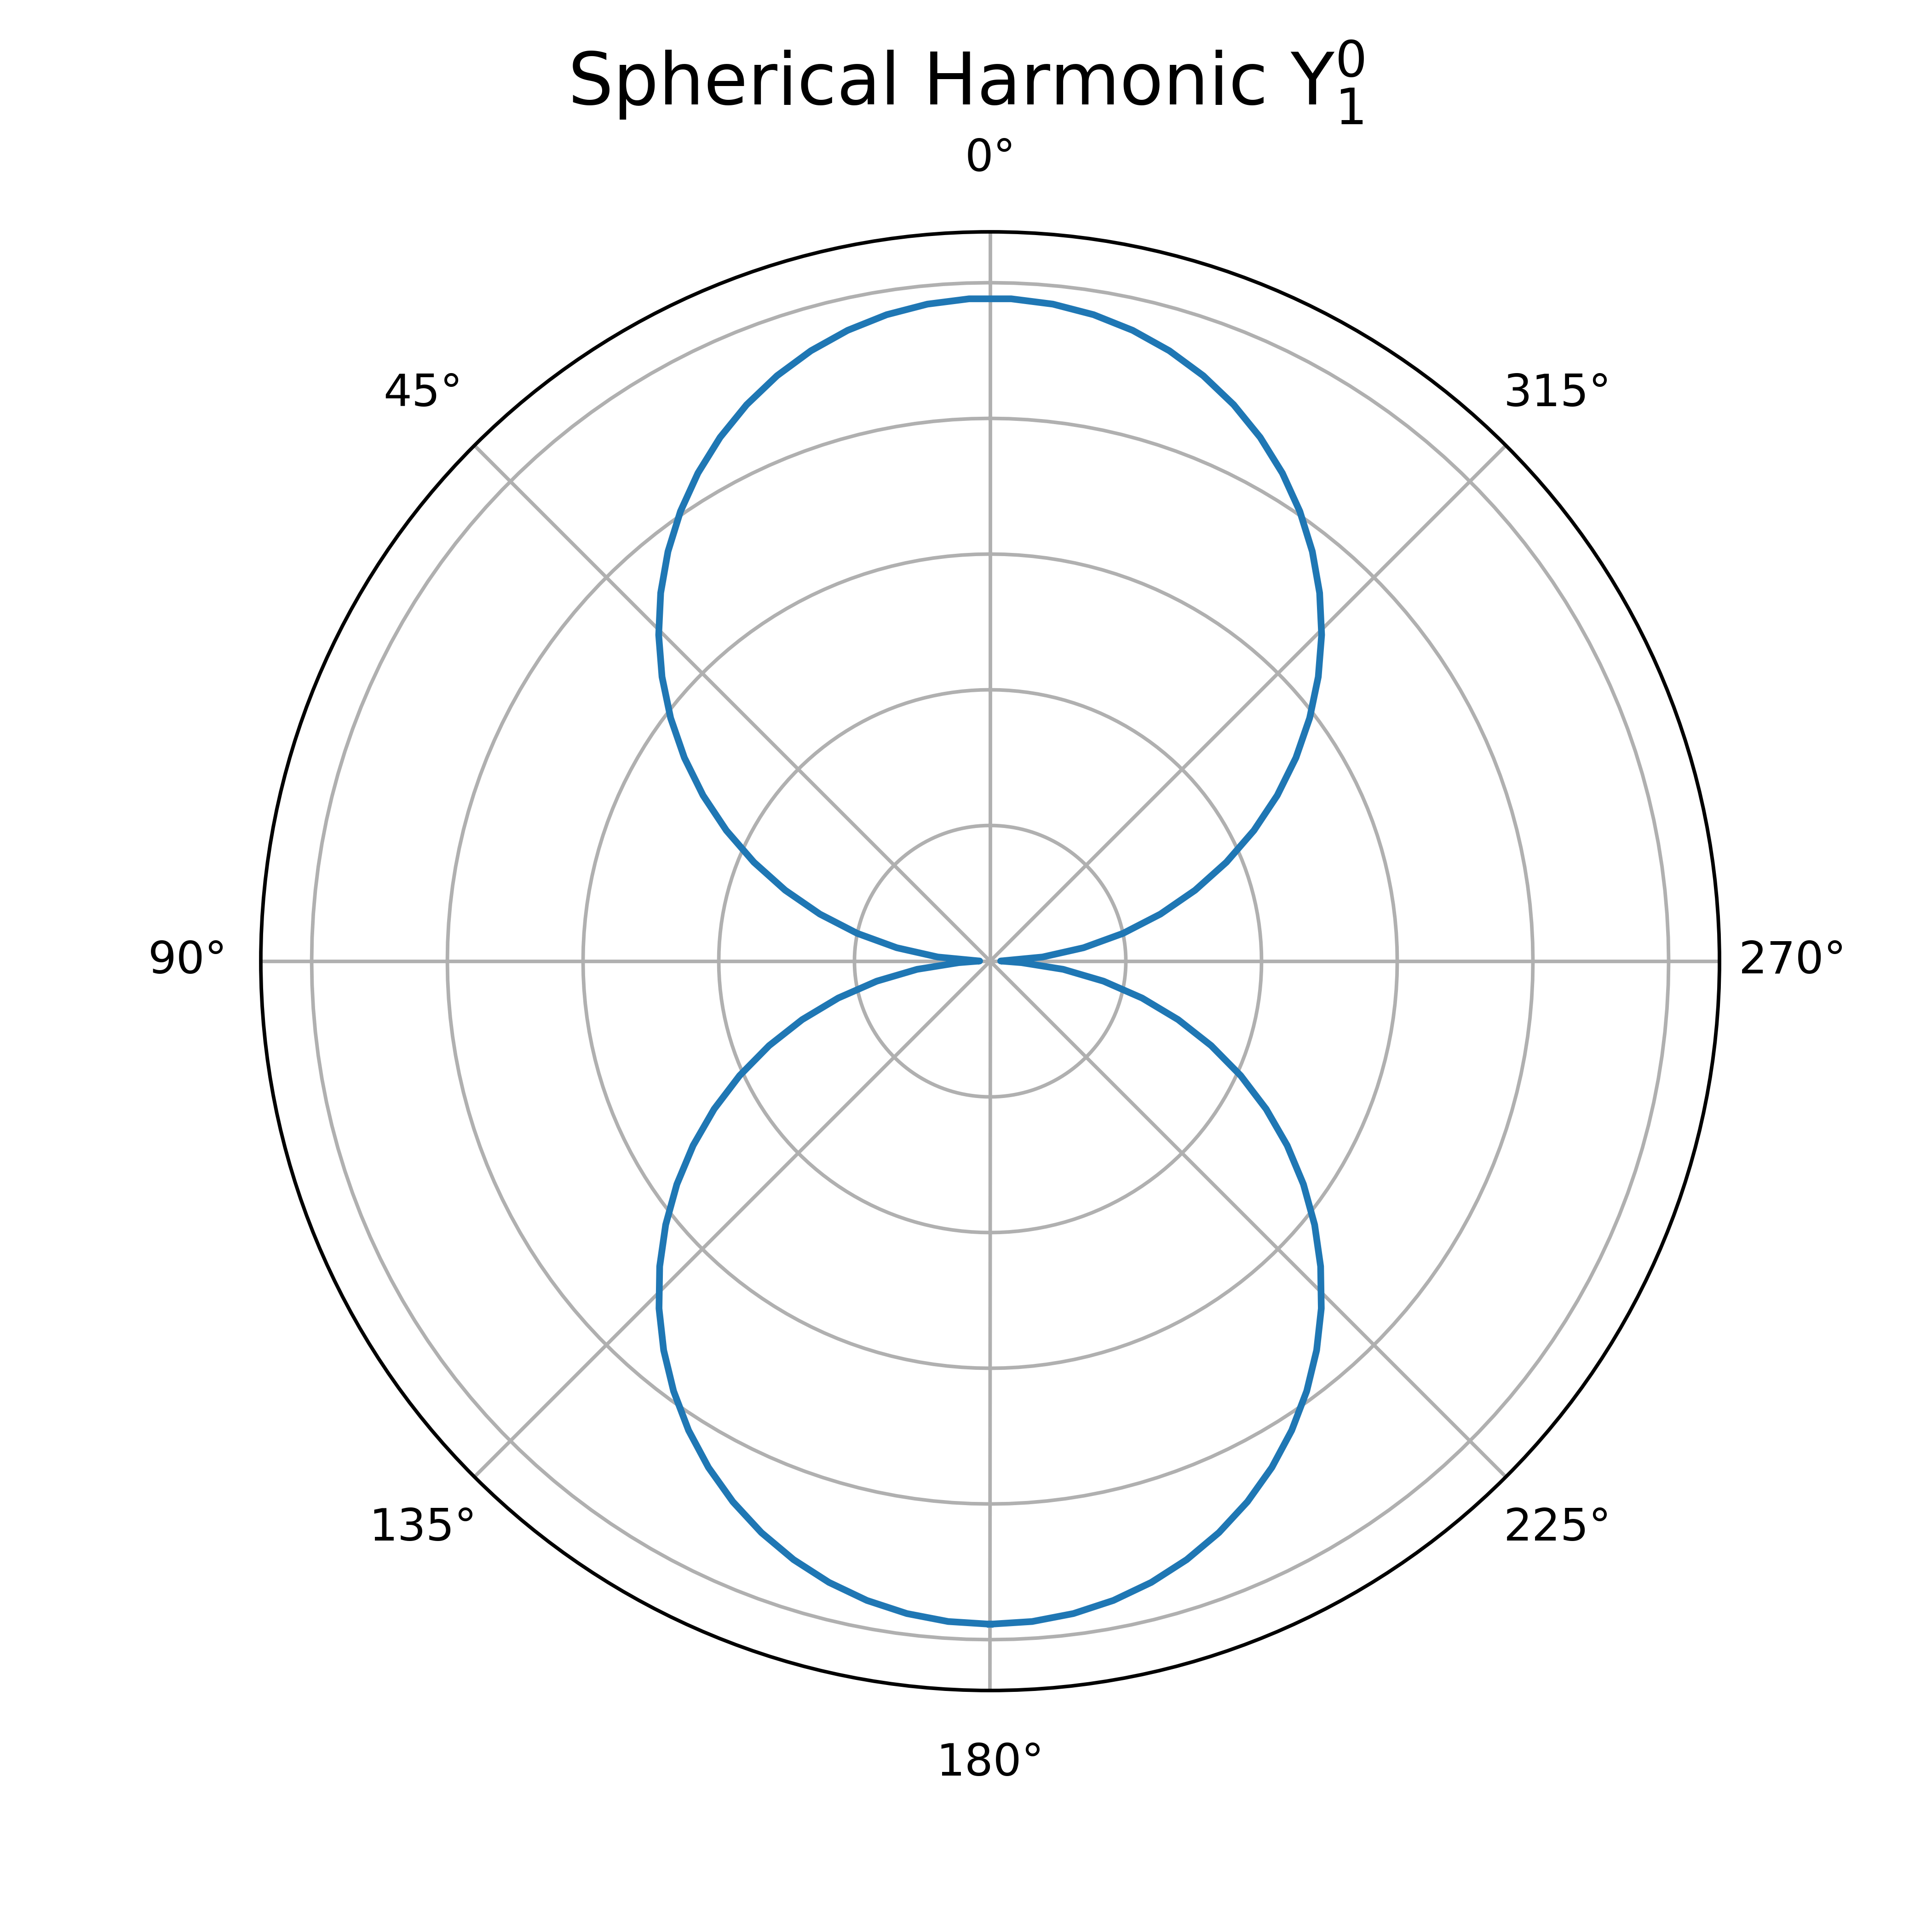
\includegraphics[width=0.4\textwidth]{SphHarm/SphHarmL1M0.png}\label{sphHarml1m0}}
		\qquad
		\subfloat[Projection of $\Ylm{1}{1}$ onto the $\varphi = 0$ plane.]{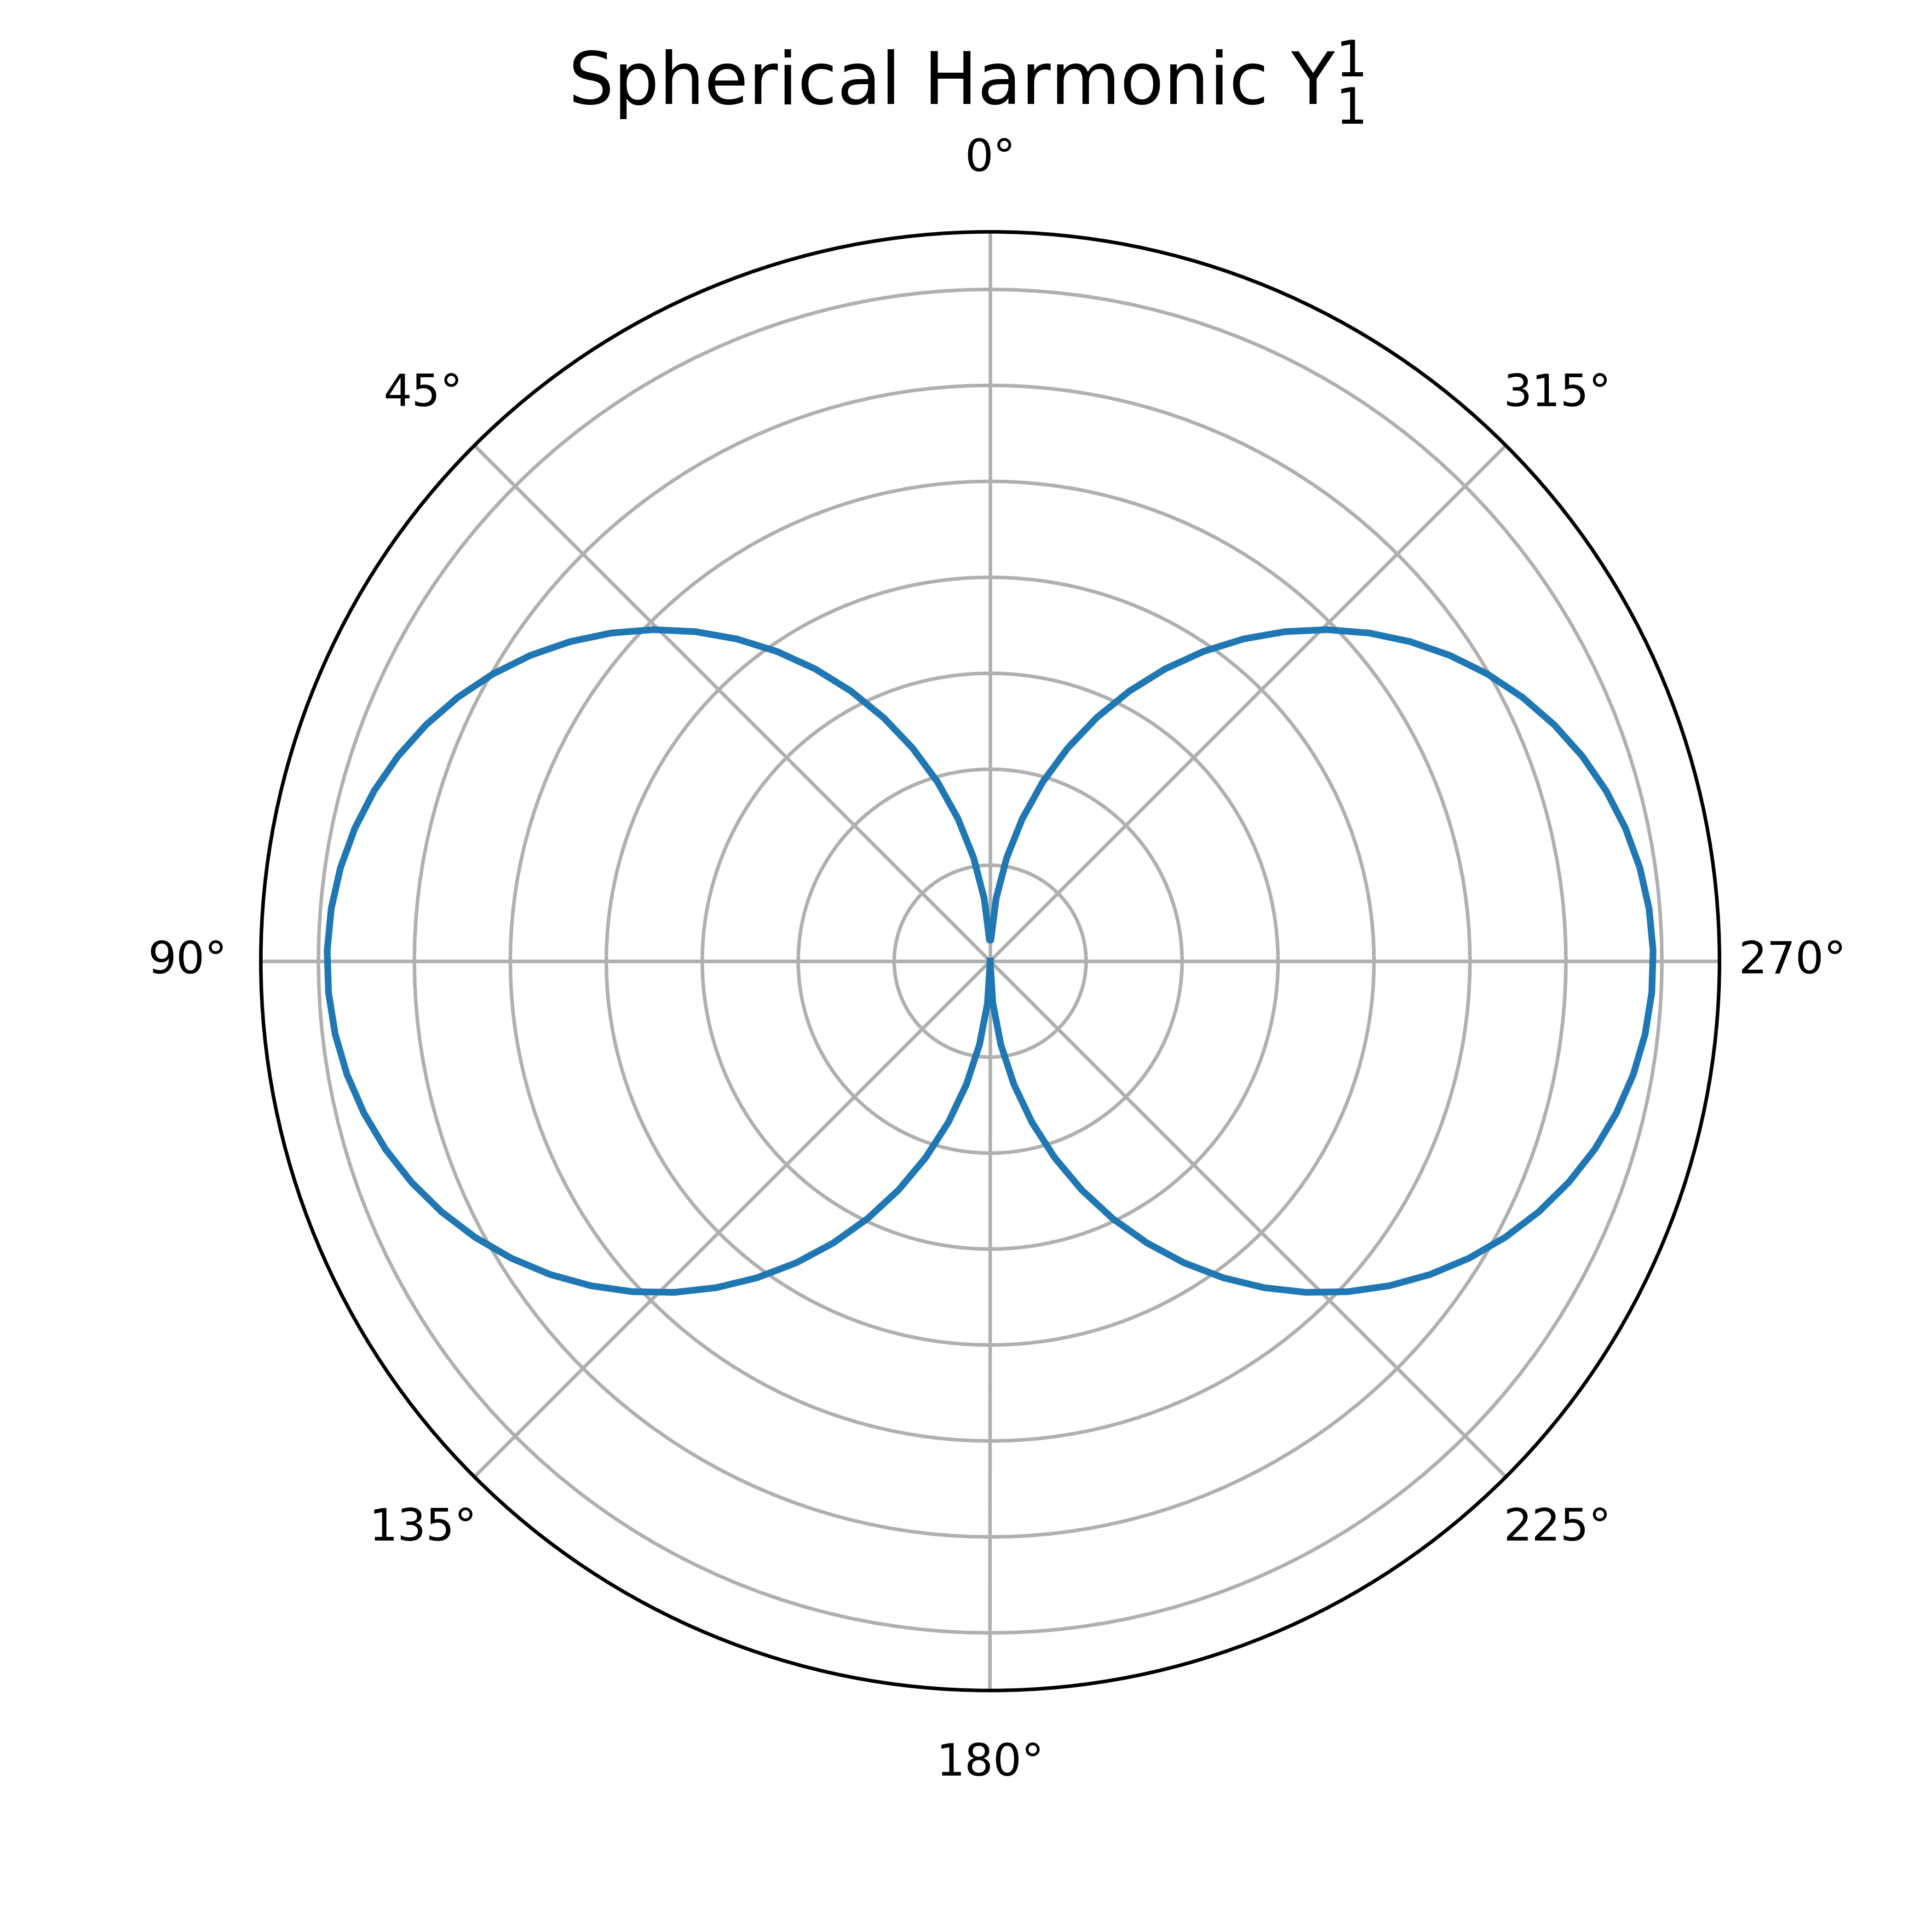
\includegraphics[width=0.4\textwidth]{SphHarm/SphHarmL1M1.png}\label{sphHarml1m1}}
		\caption{Projections of the spherical harmonics onto the $\varphi=0$ plane. Angle markings indicate polar angle $\theta$.}
		\label{L1M1Comparison}
	\end{figure}
	
	
	\section{Conclusion}
	
		\subsection{Achievements}
	
		\subsection{Error}
			
			\begin{enumerate}
				\item Angle $\alpha$ has error of $\pm 1$ Hz.
				
				\item The speaker wire was extremely sensitive to any movements. We suspect that bumping the speaker wire actually changed the angle of the speaker inside the cavity and changing the location of nodes.
			\end{enumerate}
		
	\section{Appendix: A}
	\label{AppendixA}
	
	\begin{figure}[H]
		\captionsetup{justification = raggedright}
		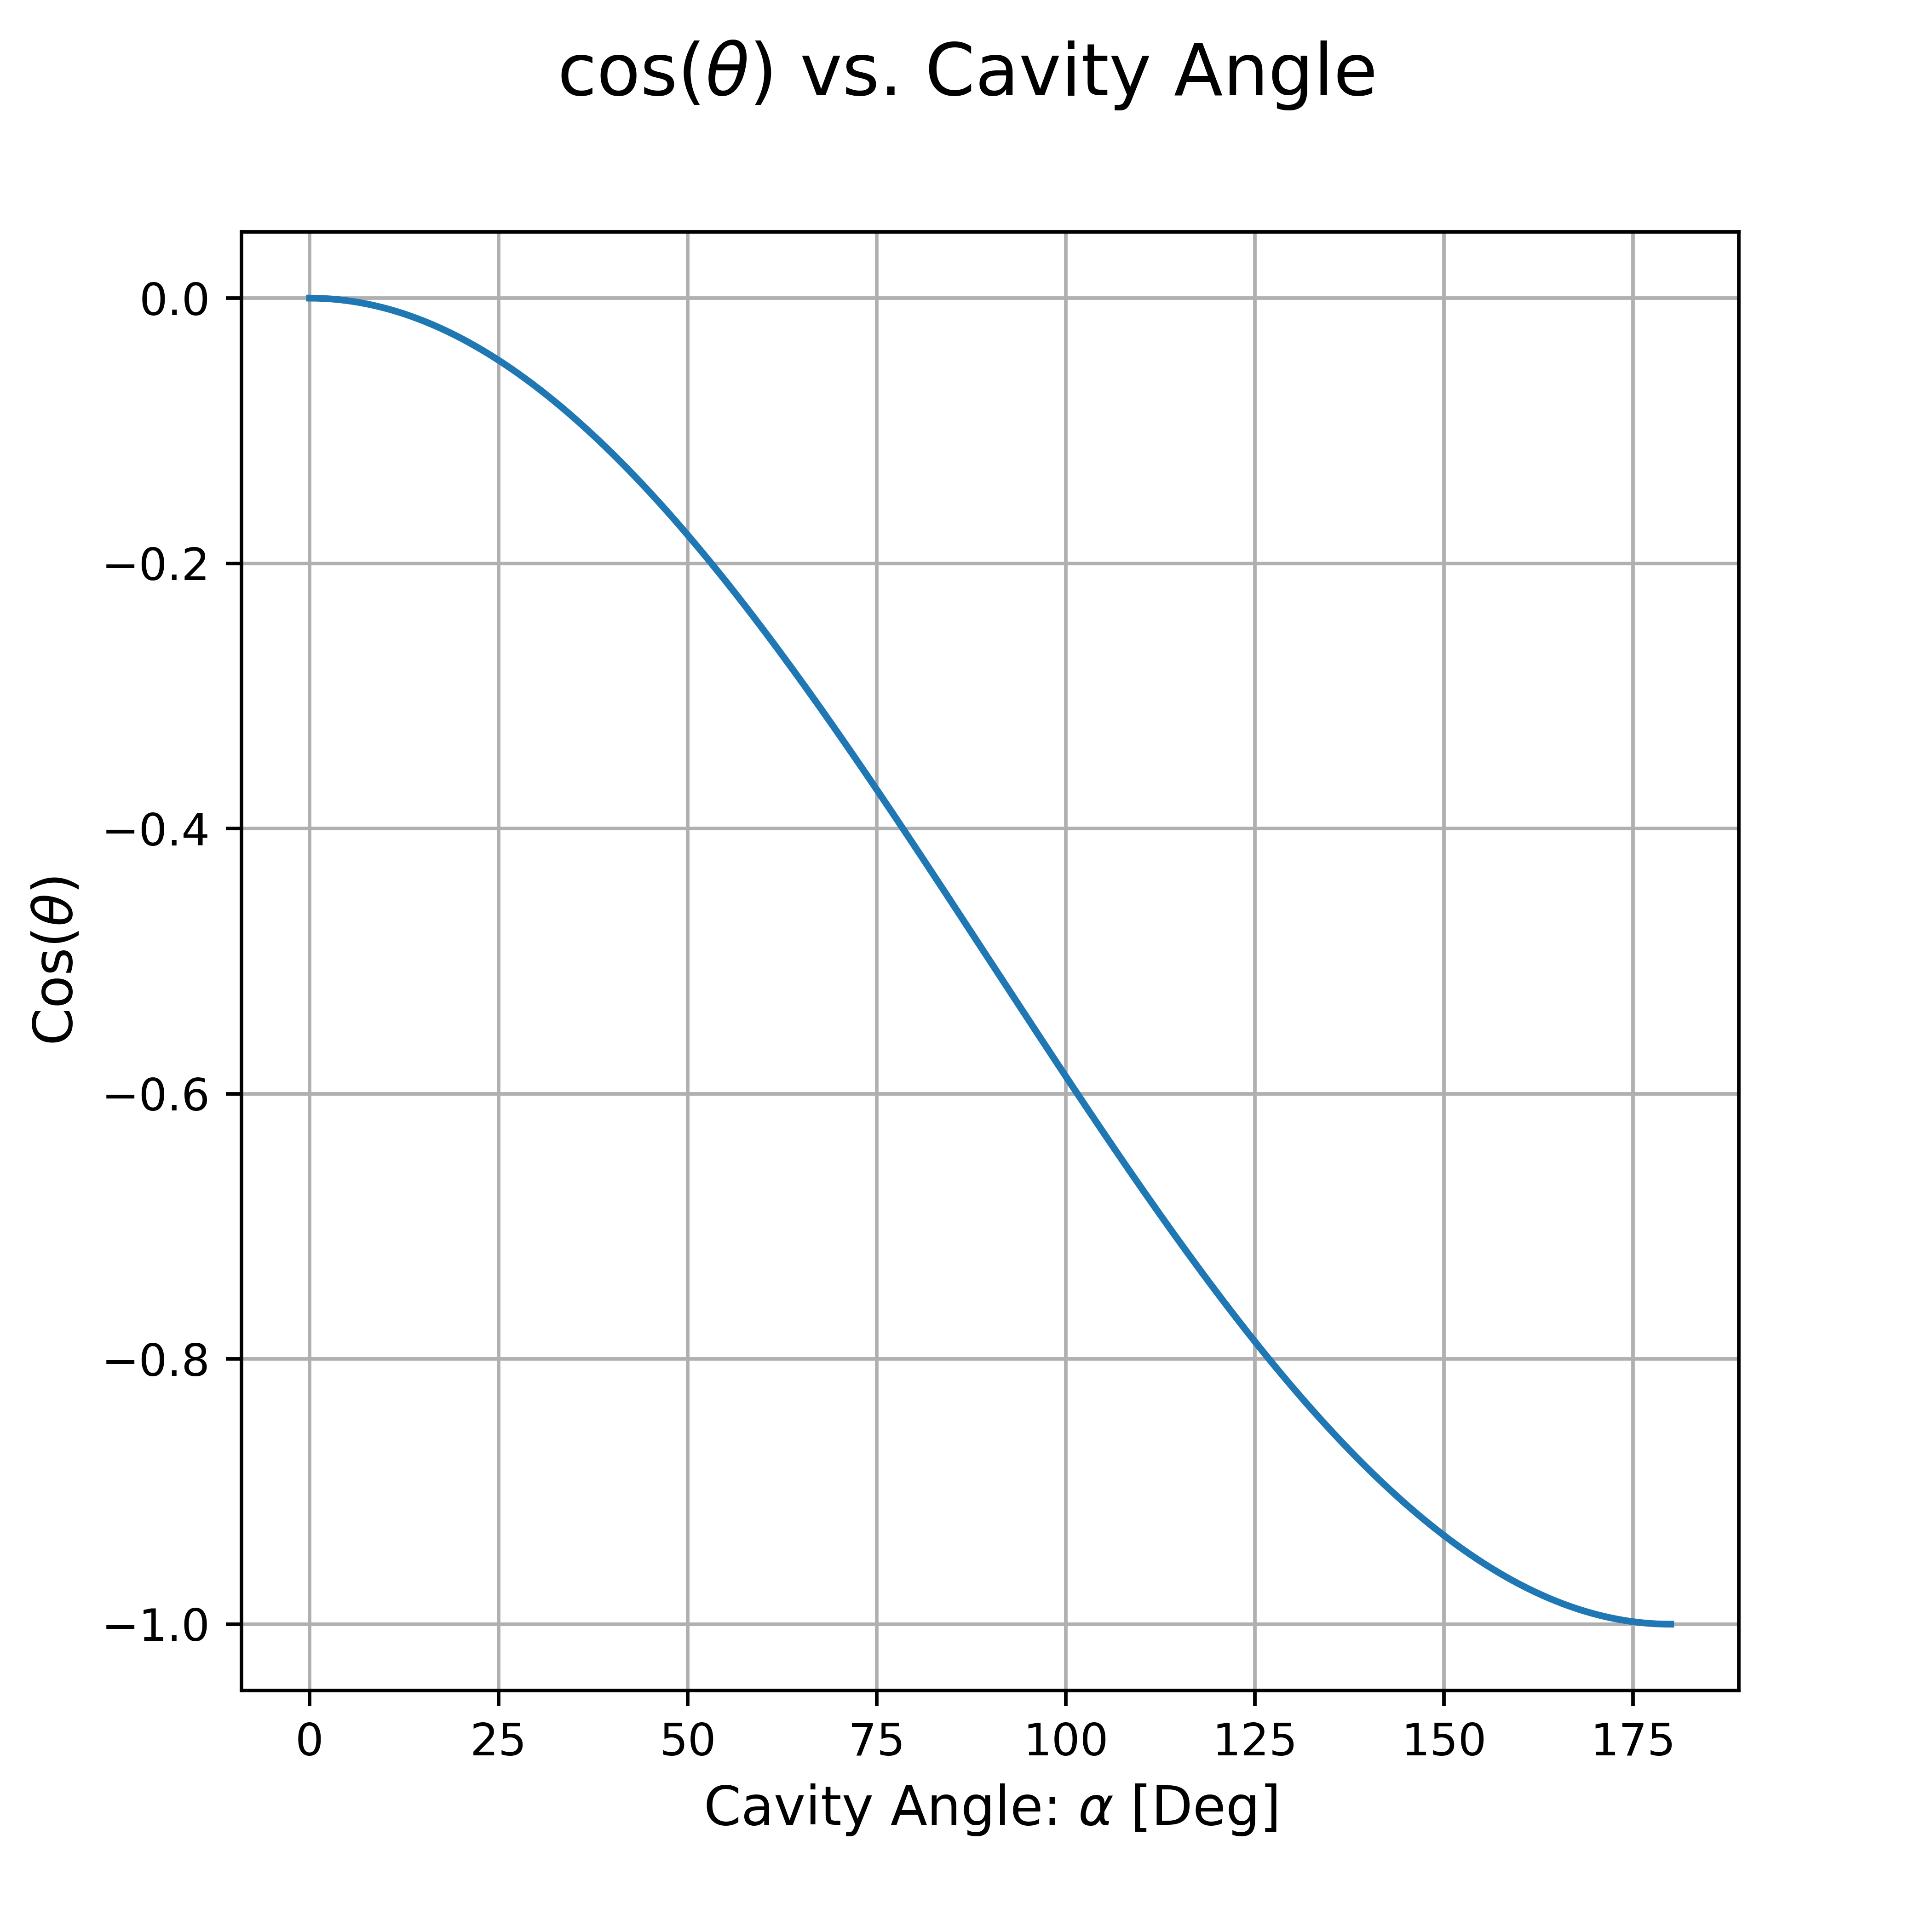
\includegraphics[width=0.4\textwidth]{Graphs/ThetaAlpha.png}
		\caption{Relation between $\cos(\theta)$ and cavity angle $\alpha$ when spherical symmetry is present}
		\label{ThetaAlpha}
	\end{figure}
	
	\pagebreak
	\subsection{Polar Angle Dependence Tables}
	
	\begin{multicols}{2}
		\begin{table}[H]
			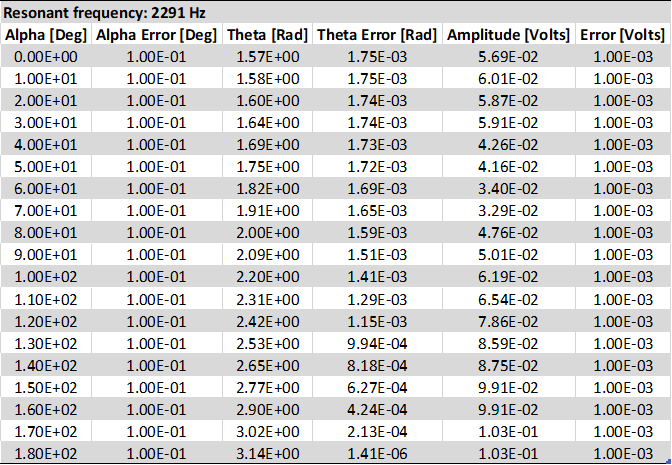
\includegraphics[width=0.45\textwidth]{Tables/2291Table.png}
			\caption{Data table for resonant frequency $2291$ Hz.}
			\label{2291Table}		
		\end{table} 
	\columnbreak
		\begin{figure}[H]
			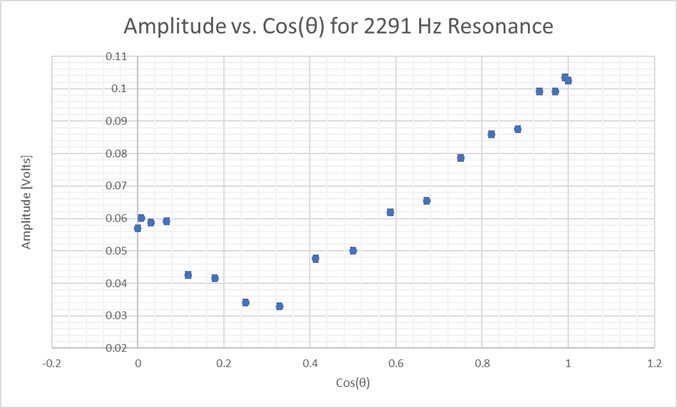
\includegraphics[width=0.45\textwidth]{Graphs/2291Graph.png}
			\caption{Graph of \cref{2291Table}. We can clearly see a single node at $\theta = 1.91$ radians.}
			\label{2291Graph}
		\end{figure}
	\end{multicols}
	
	\begin{multicols}{2}
			\begin{table}[H]
			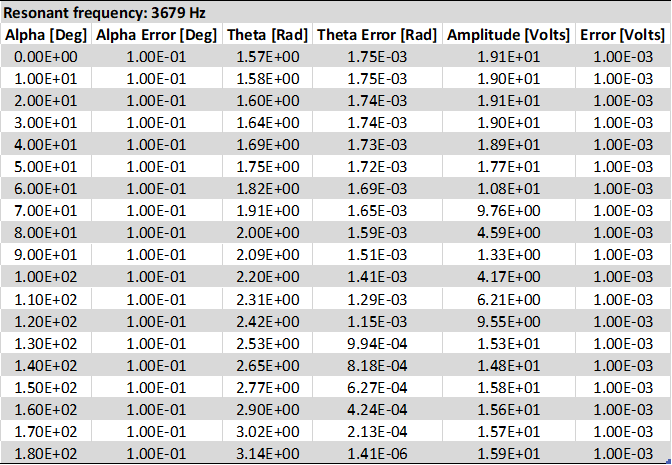
\includegraphics[width=0.45\textwidth]{Tables/3679Table.png}
			\caption{Table showing amplitude vs polar angle for 3679 Hz resonance.}
			\label{3679Table}		
		\end{table} 
	\columnbreak
		\begin{figure}[H]
			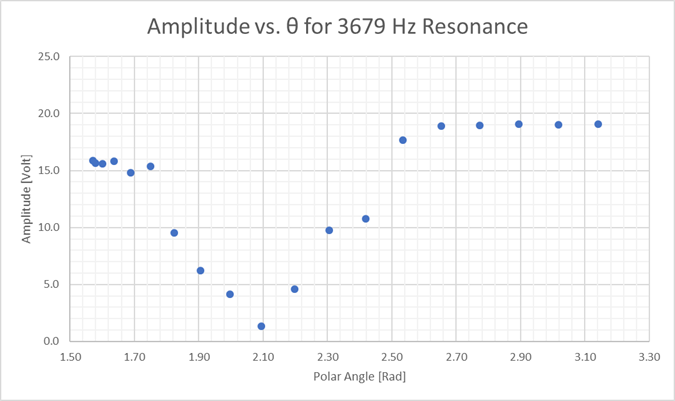
\includegraphics[width=0.45\textwidth]{Graphs/3679Graph.png}
			\caption{Graph of \cref{3679Table}. We can clearly see a single node at $\theta = 2.09$ radians.}
			\label{3679Graph}
		\end{figure}
	\end{multicols}
	
	\begin{multicols}{2}	
		\begin{table}[H]
			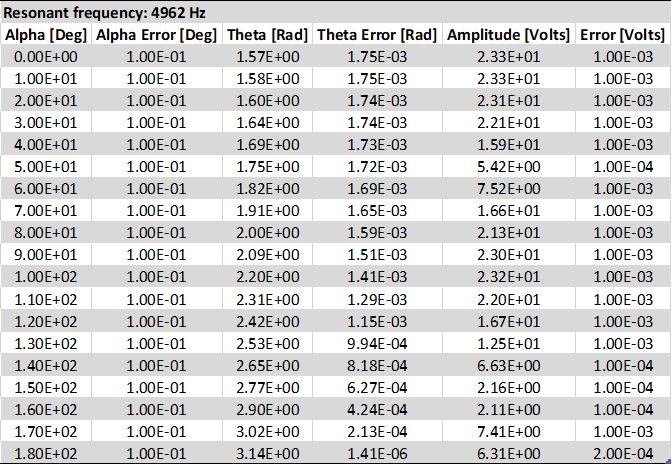
\includegraphics[width=0.45\textwidth]{Tables/4962Table.png}
			\caption{Table showing amplitude vs polar angle for 4926 Hz resonance.}
			\label{4962Table}		
		\end{table}
	\columnbreak
		\begin{figure}[H]
			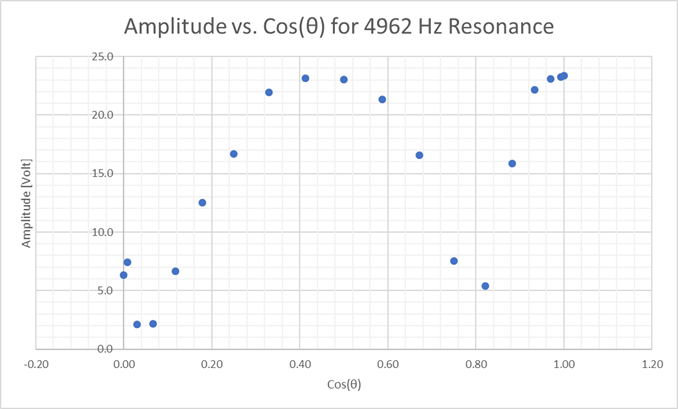
\includegraphics[width=0.45\textwidth]{Graphs/4962Graph.png}
			\caption{Graph of \cref{4962Table}. We can clearly see a single node at $\theta = $ radians.}
			\label{4962Graph}
		\end{figure}
	\end{multicols}


	\begin{multicols}{2}	
		\begin{table}[H]
			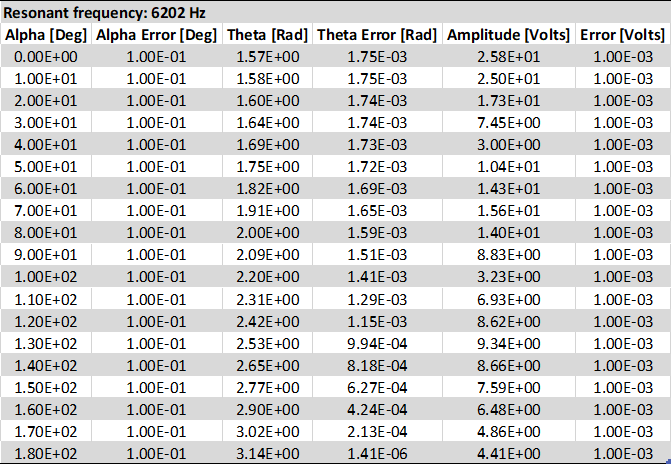
\includegraphics[width=0.45\textwidth]{Tables/6202Table.png}
			\caption{Table showing amplitude vs polar angle for 6202 Hz resonance.}
			\label{6202Table}		
		\end{table}
	\columnbreak
		\begin{figure}[H]
			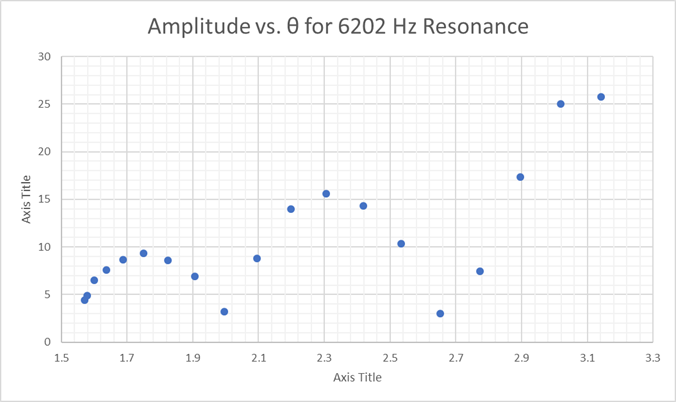
\includegraphics[width=0.45\textwidth]{Graphs/6202Graph.png}
			\caption{Graph of \cref{6202Table}. We can clearly see a single node at $\theta = $ radians.}
			\label{6202Graph}
		\end{figure}
	\end{multicols}


	\begin{multicols}{2}	
		\begin{table}[H]
			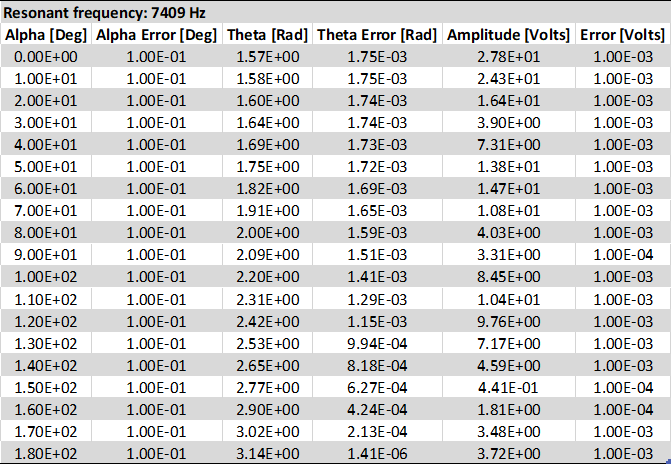
\includegraphics[width=0.45\textwidth]{Tables/7409Table.png}
			\caption{Table showing amplitude vs polar angle for 7409 Hz resonance.}
			\label{7409Table}		
		\end{table}
	\columnbreak
		\begin{figure}[H]
			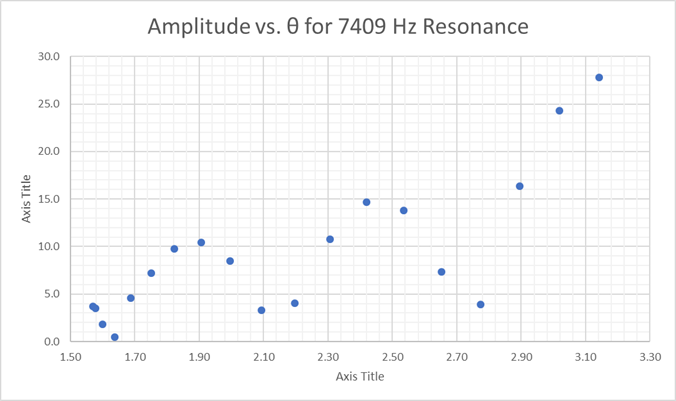
\includegraphics[width=0.45\textwidth]{Graphs/7409Graph.png}
			\caption{Graph of \cref{7409Table}. We can clearly see a single node at $\theta = $ radians.}
			\label{7409Graph}
		\end{figure}
	\end{multicols}

	\subsection{Spherical Harmonics}
	
		\begin{figure}[H]
		\centering
		\subfloat[Spherical harmonic for $\ell = 1$, $m= 0$]{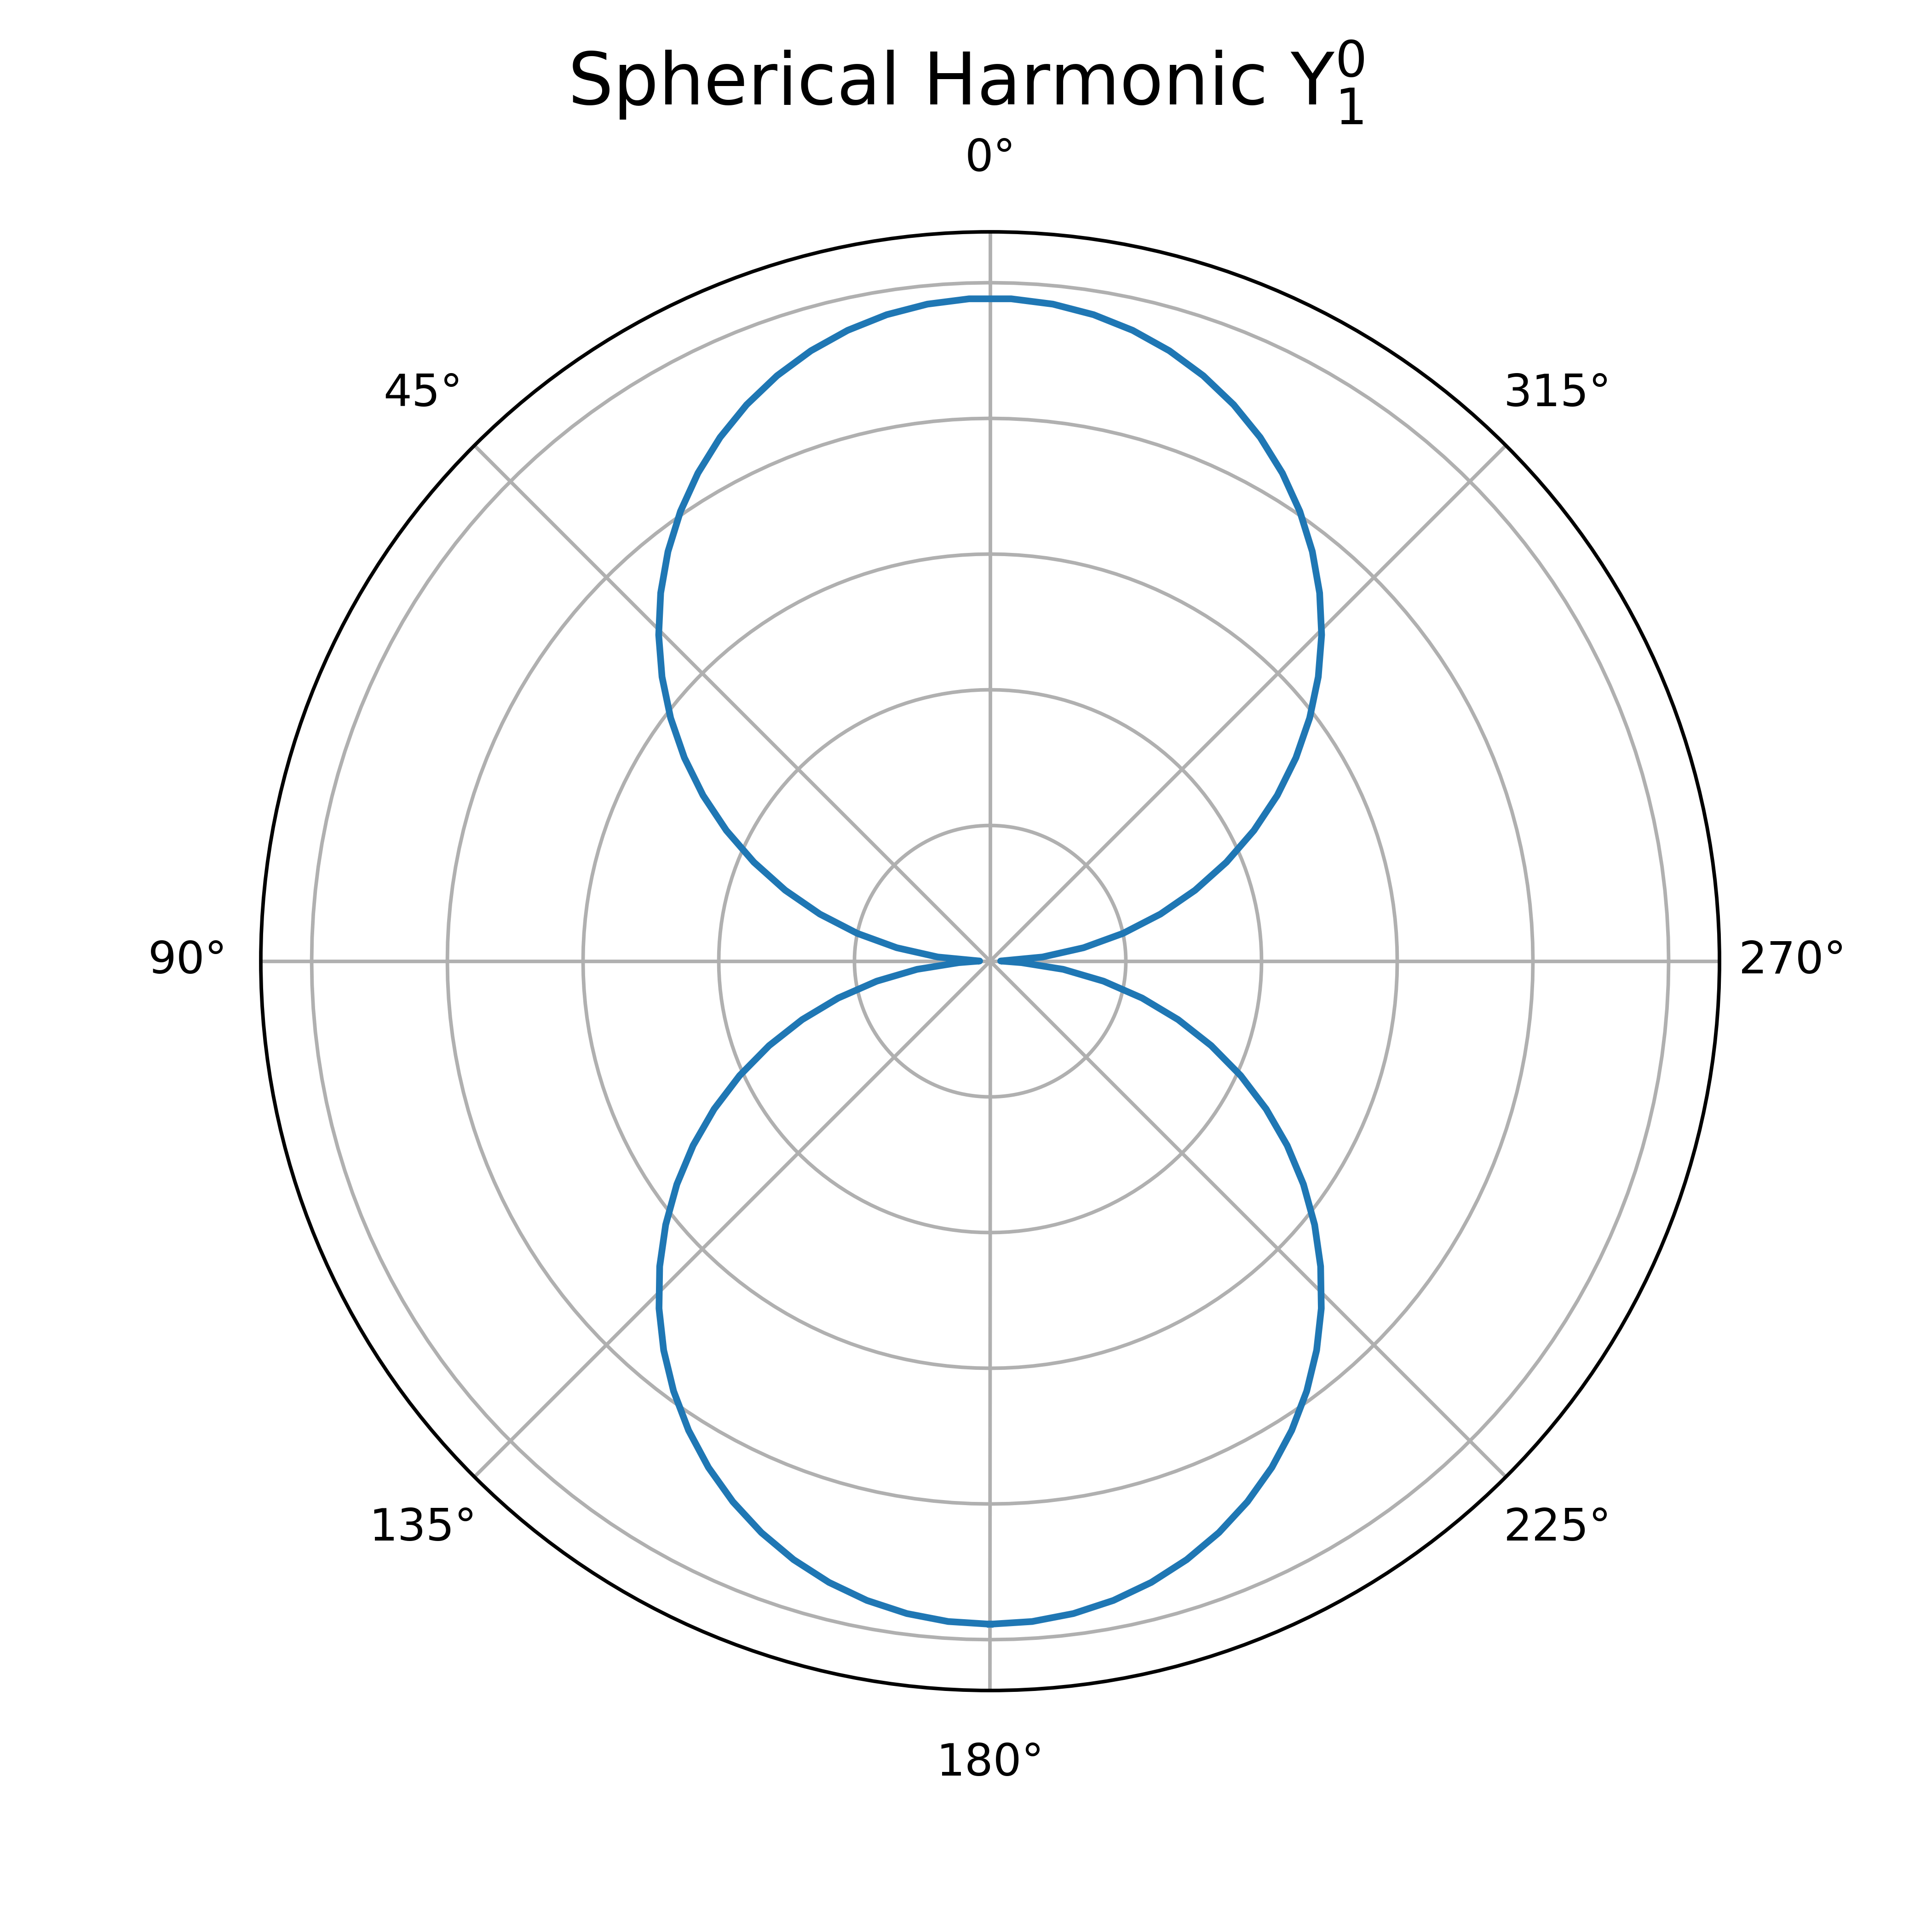
\includegraphics[width=0.4\textwidth]{SphHarm/SphHarmL1M0.png}\label{sphHarmL1M0}}
		\qquad
		\subfloat[Spherical harmonic for $\ell = 2$, $m=0$]{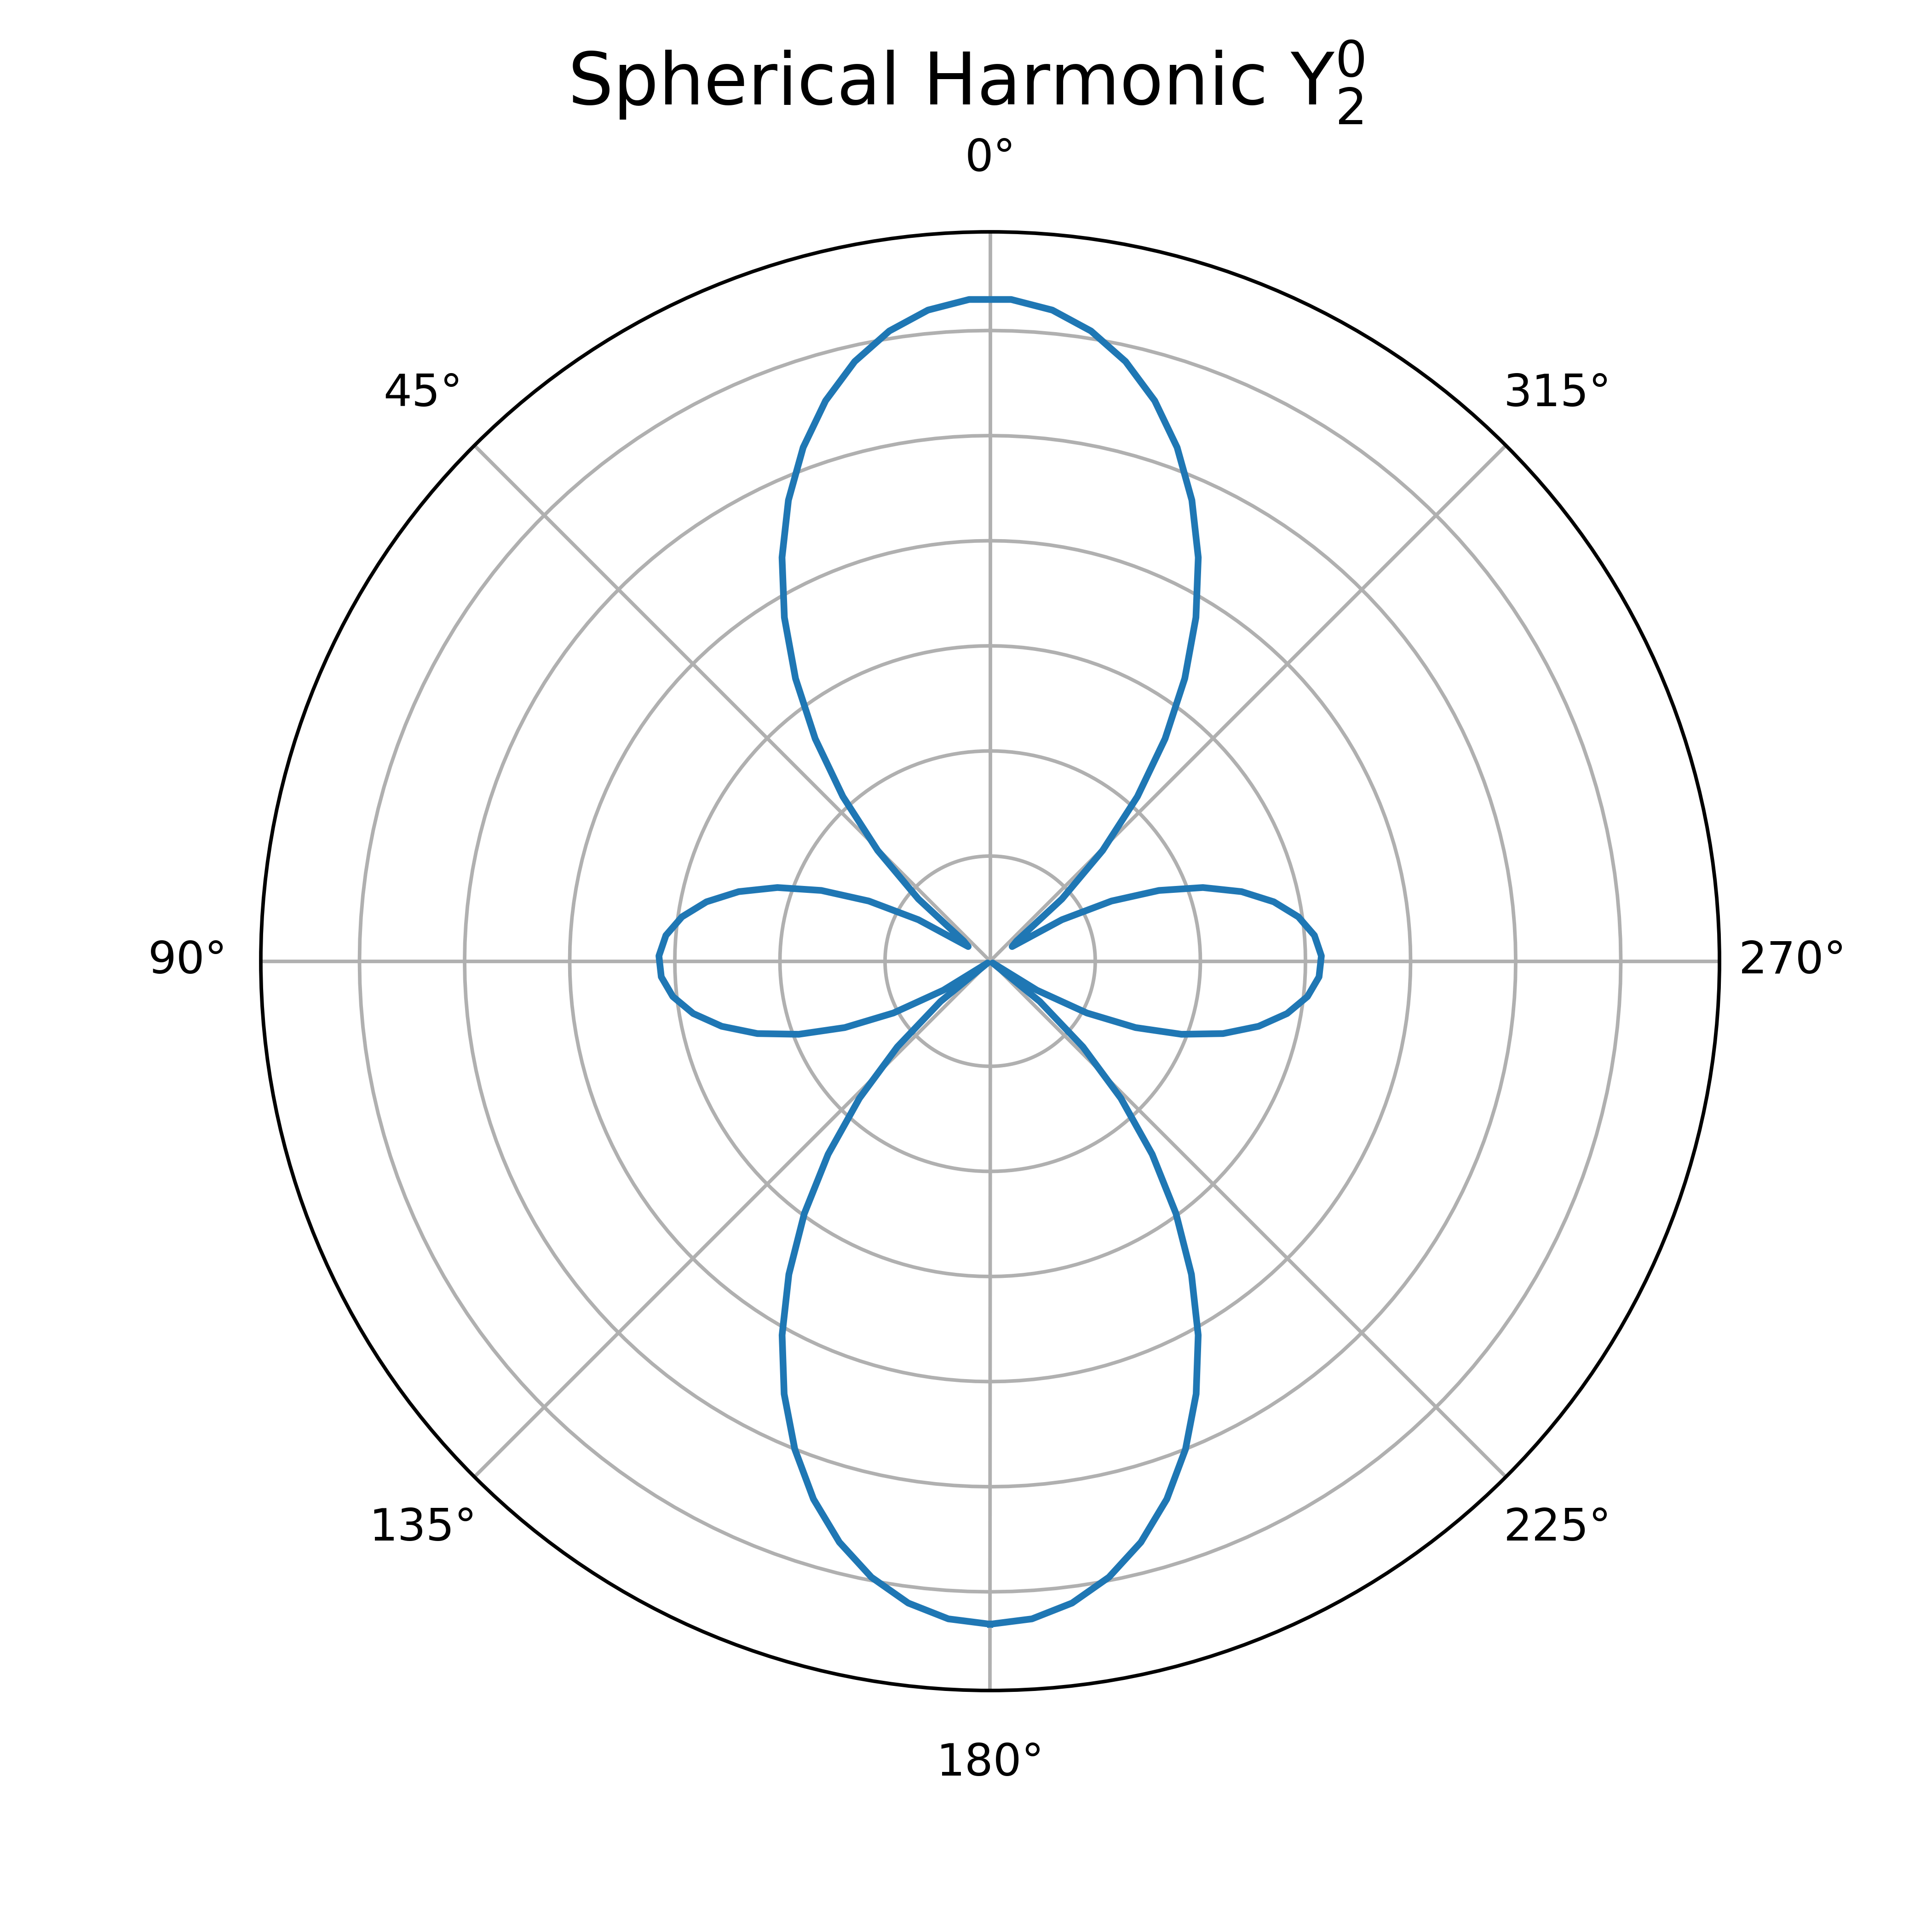
\includegraphics[width=0.4\textwidth]{SphHarm/SphHarmL2M0.png}\label{sphHarmL2M0}}
		\\
		\subfloat[Spherical harmonic for $\ell = 3$, $m = 0$]{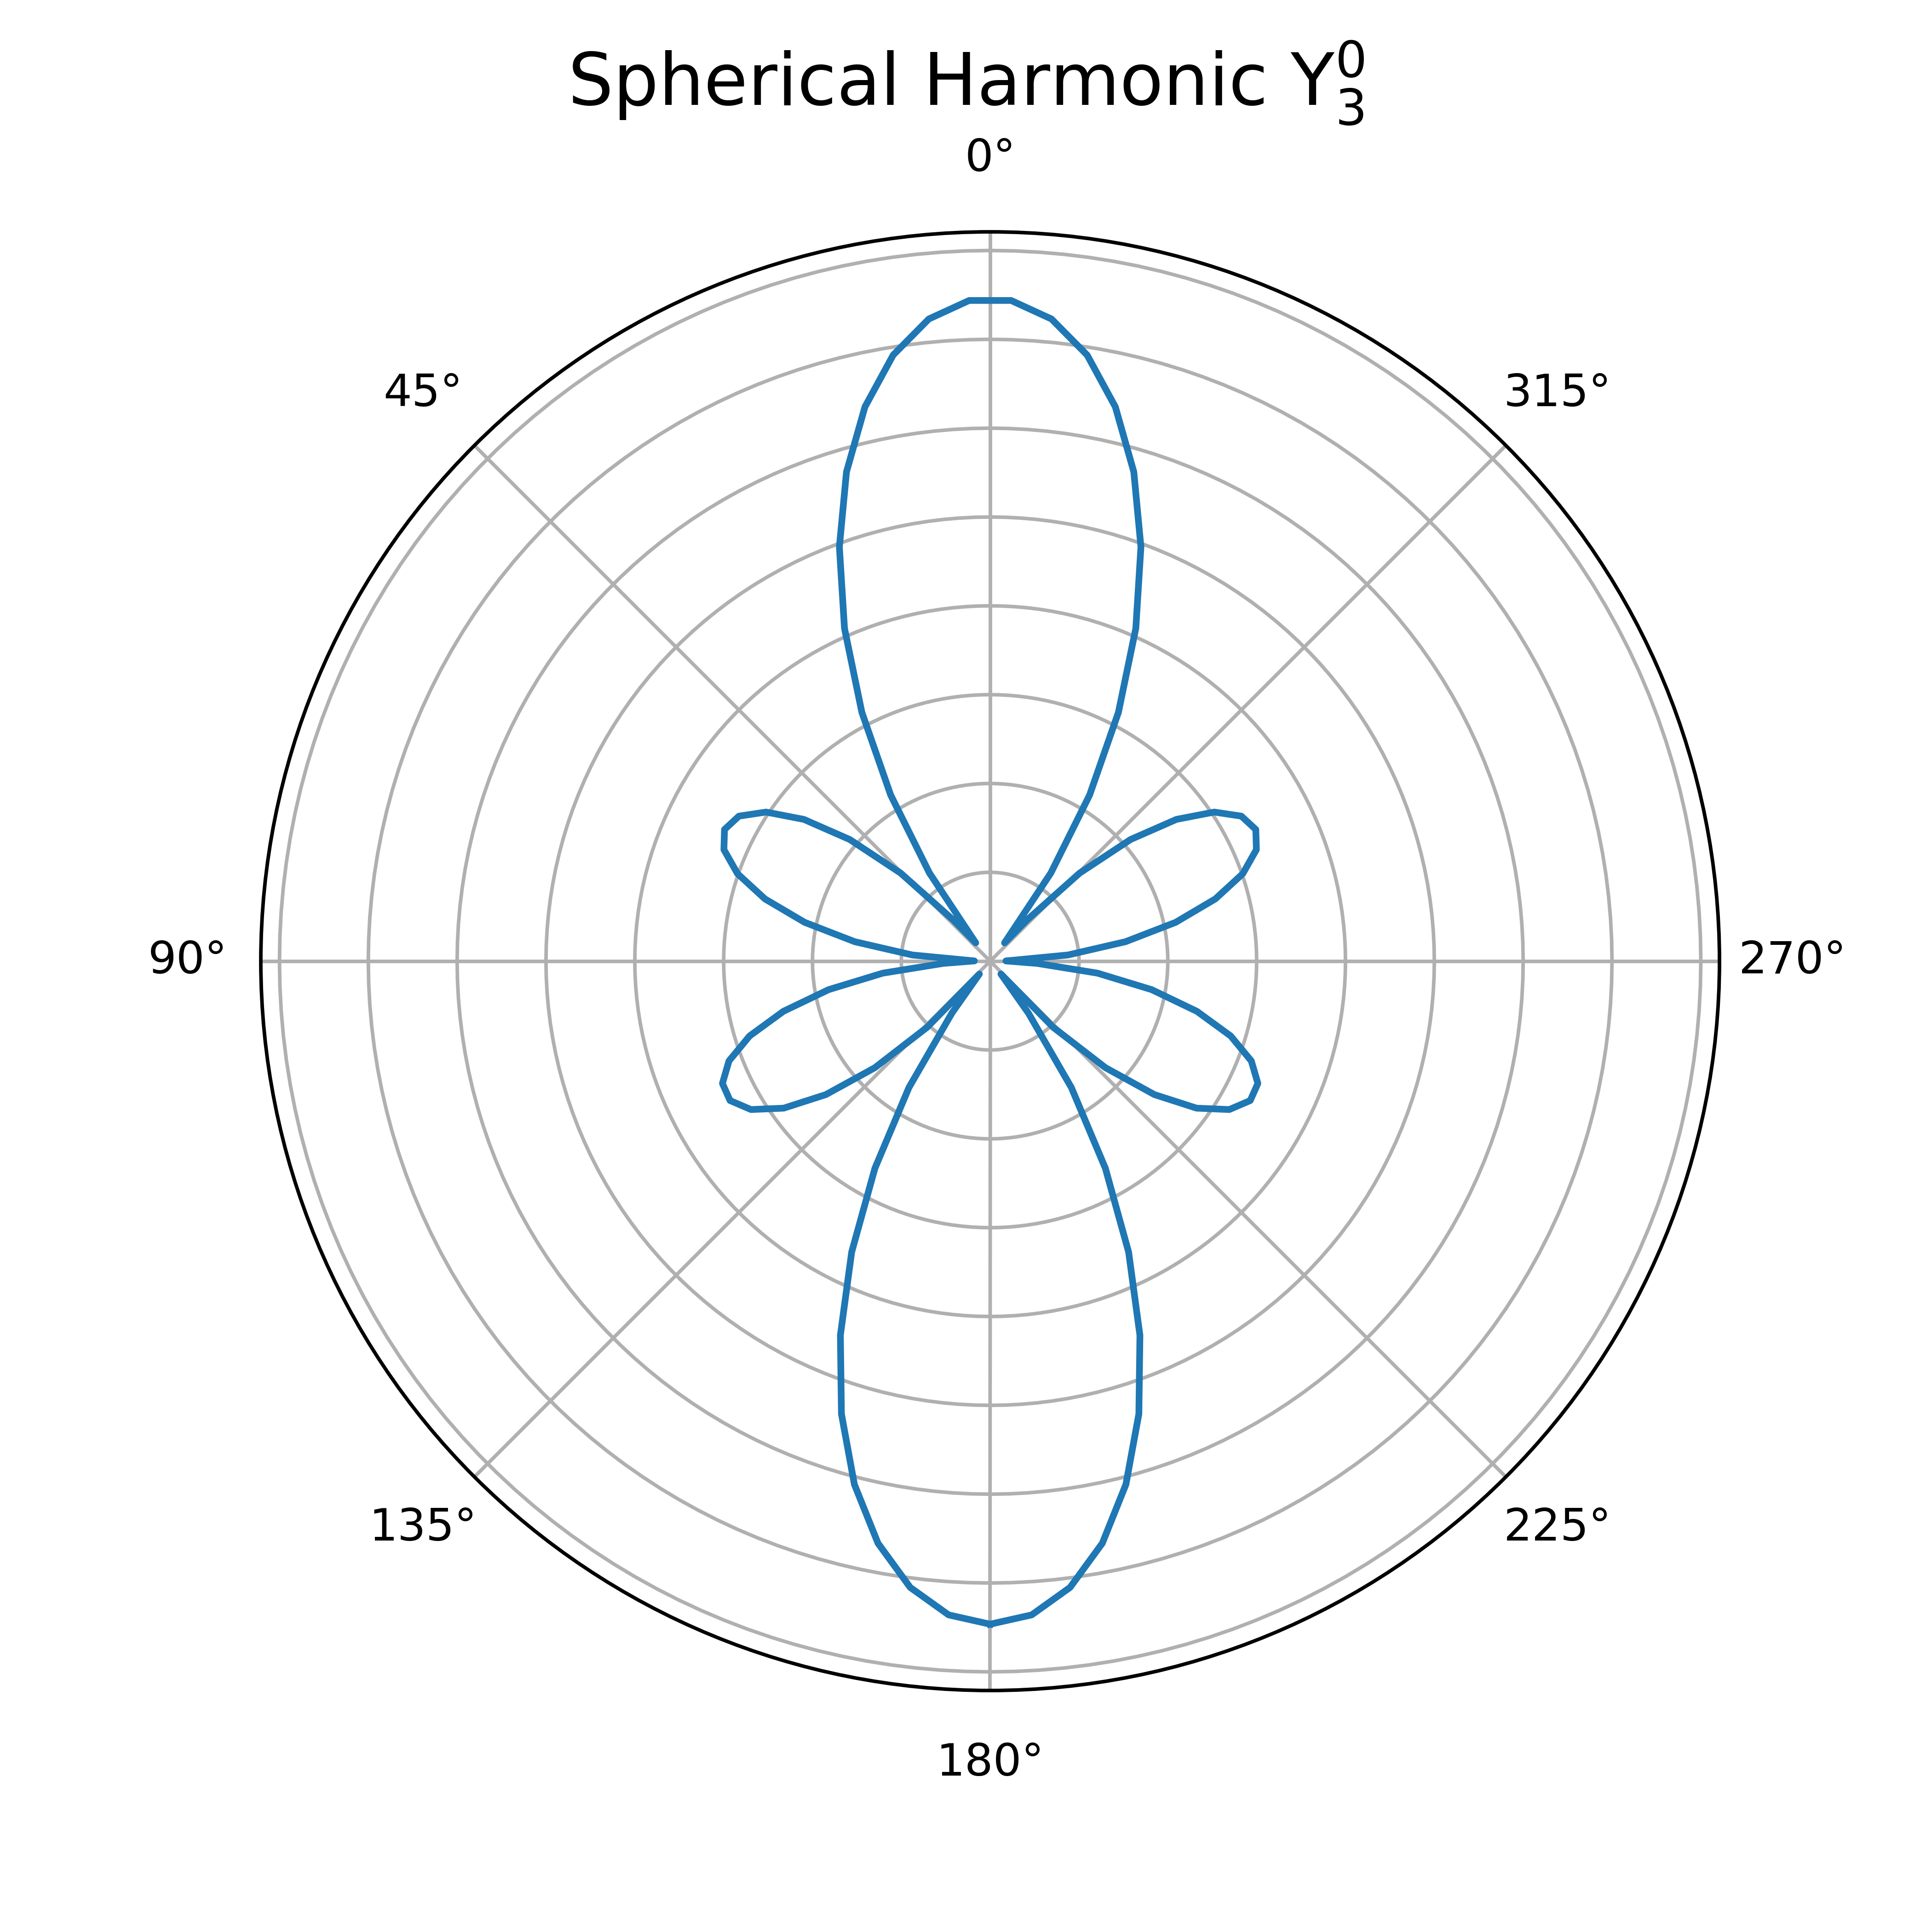
\includegraphics[width=0.4\textwidth]{SphHarm/SphHarmL3M0.png}\label{sphHarmL3M0}}
		\qquad
		\subfloat[Spherical harmonic for $\ell = 5$, $m = 1$]{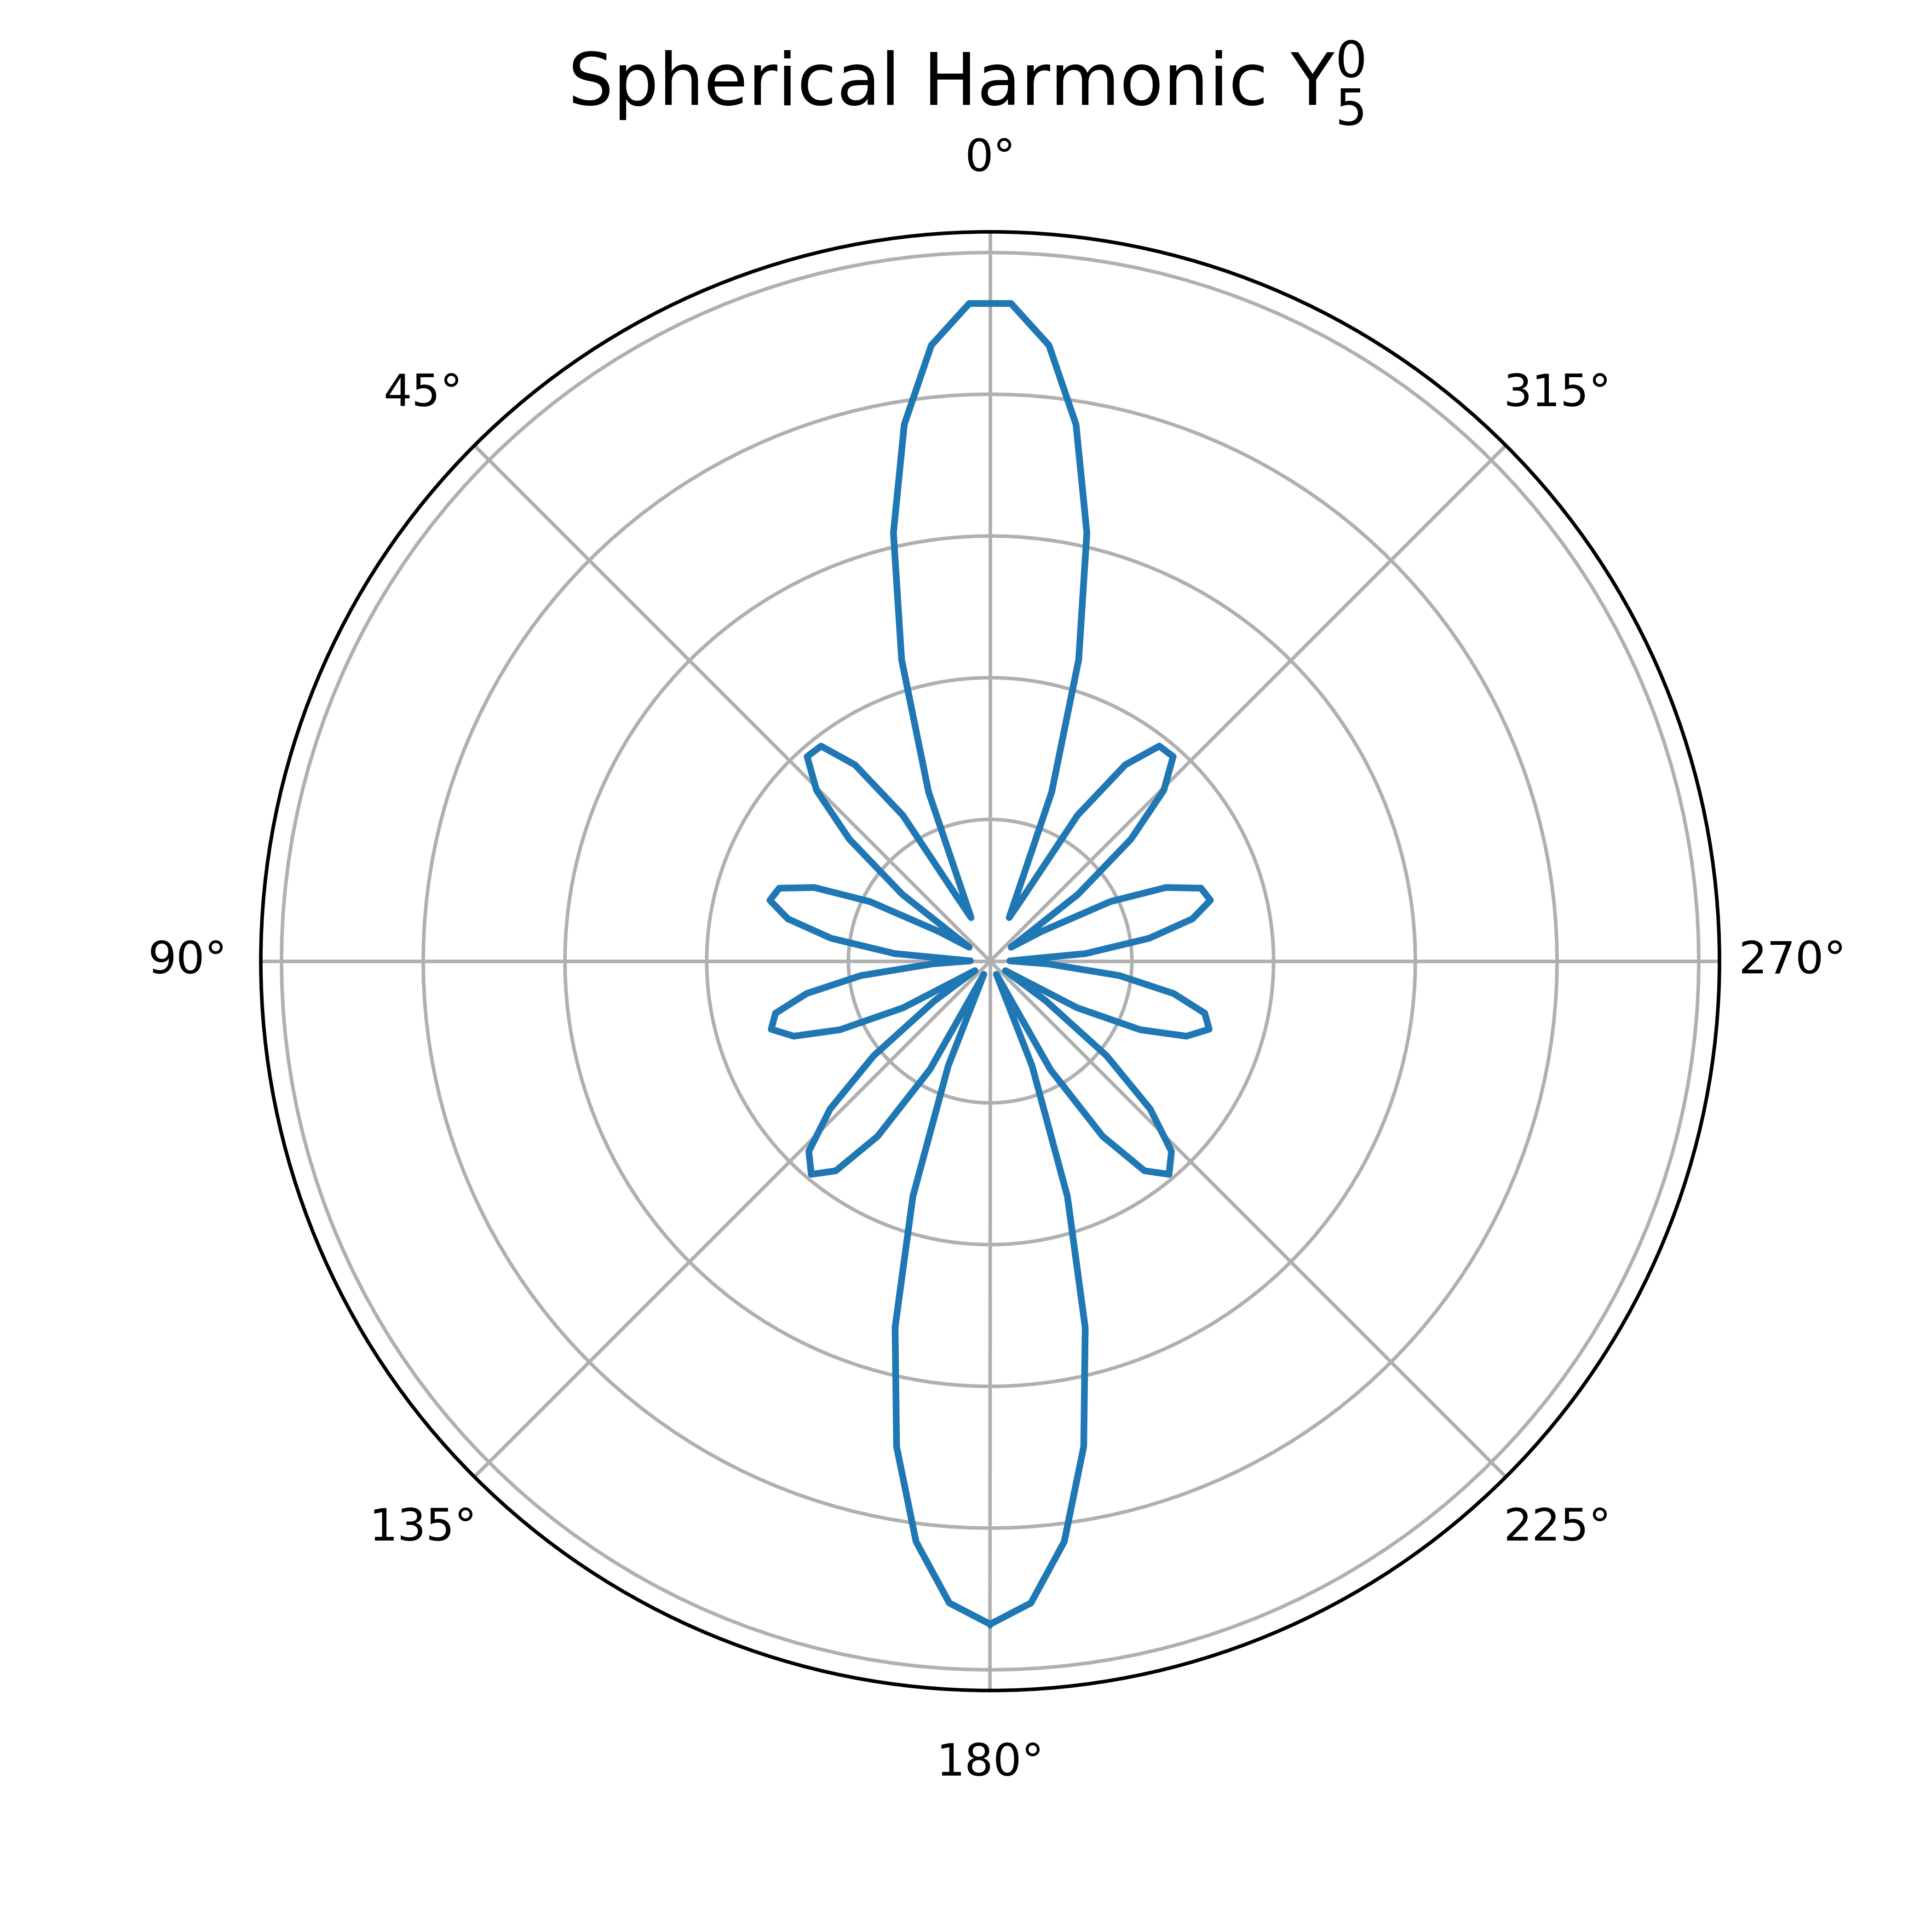
\includegraphics[width=0.4\textwidth]{SphHarm/SphHarmL5M0.png}\label{sphHarmL5M0}}
		\caption{Spherical Harmonics $\mathrm{Y}^\ell_m$ with azimuthal angle $\varphi = 0$.}
		\label{sphereHarm}
	\end{figure}
	
	\subsection{Broken Cavity Symmetry}
	
	\subsection{3mm Spacing}
	\begin{figure}[H]
		\centering
		\subfloat[Caption A ]{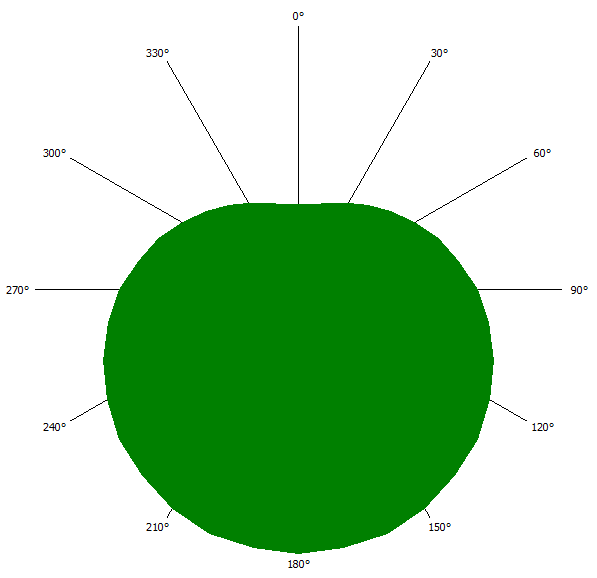
\includegraphics[width=0.4\textwidth]{Day4/L13mmPolar2084_806.png}}
		\qquad
		\subfloat[Caption B]{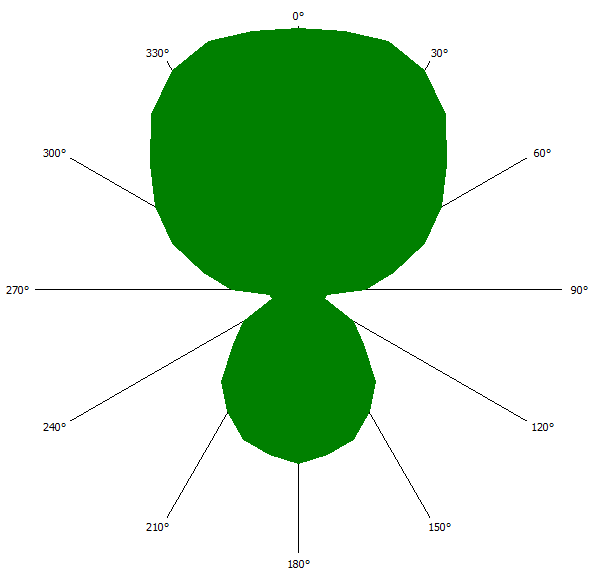
\includegraphics[width=0.4\textwidth]{Day4/L13mmPolar2251_140.png}}
		\caption{3mm Spacing}
		\label{3mmliftedDegeneracy}
	\end{figure}


	\begin{figure}[H]
		\centering
		\subfloat[Caption A ]{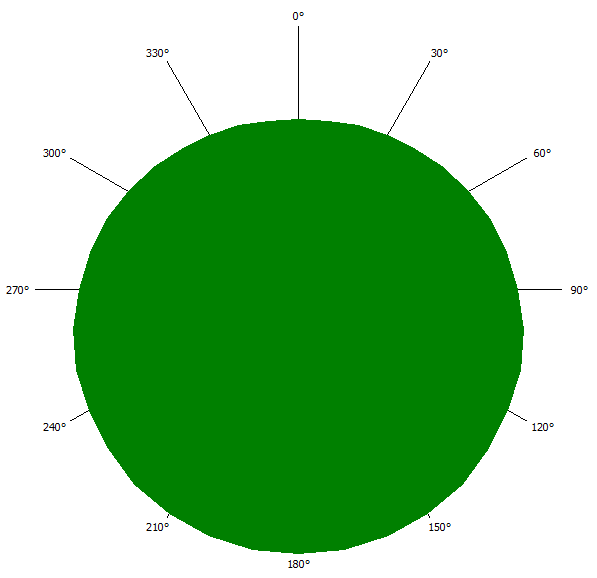
\includegraphics[width=0.4\textwidth]{Day4/L16mmPolar2084_806.png}}
		\qquad
		\subfloat[Caption B]{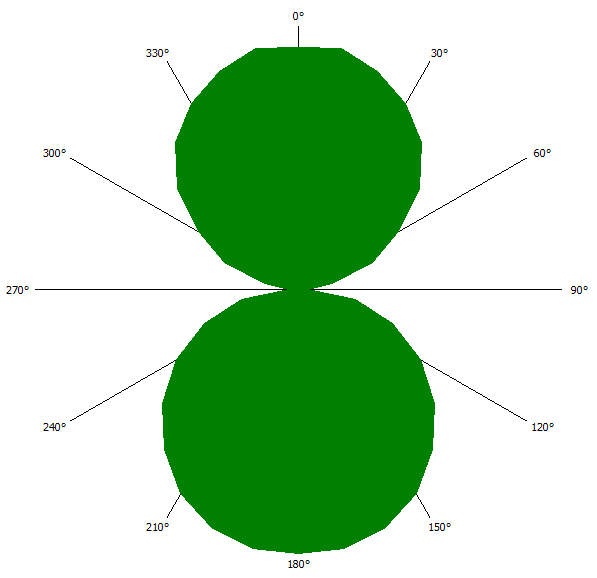
\includegraphics[width=0.4\textwidth]{Day4/L16mmPolar2251_140.png}}
		\caption{3mm Spacing}
		\label{6mmliftedDegeneracy}
	\end{figure}


%	\begin{figure}[H]
%		\centering
%		\subfloat[$\ell=2$, $m=-1$ resonance]{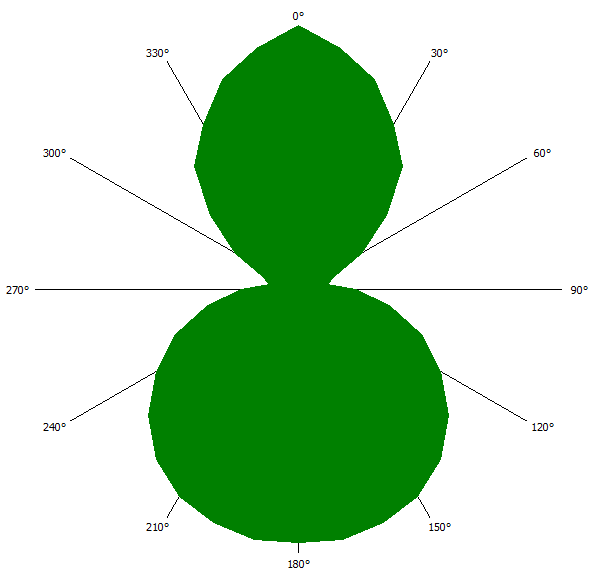
\includegraphics[width=0.3\textwidth]{2.3.3/3mmPolar/323_Polar_L1M-1Amp_freq3591_549.png} \label{3-0mmDegeneracy}}
%		\quad
%		\subfloat[$\ell=2$, $m=0$ resonance]{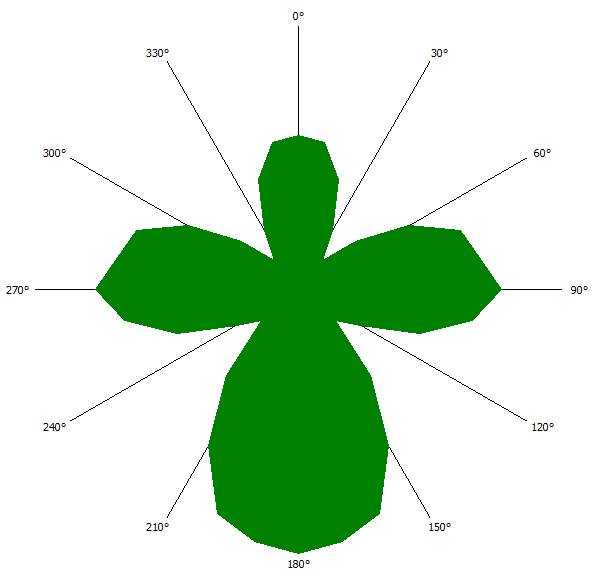
\includegraphics[width=0.3\textwidth]{2.3.3/3mmPolar/323_Polar_L1M1Amp_freq3647_513.png} \label{3-1mmDegeneracy}}
%		\caption{Polar plots of lifted degeneracies for 3mm spacing}
%		\label{3mmliftedDegeneracy}
%	\end{figure}
%	It is important to note that not all the degeneracies were lifted at $3$ mm spacing.


%
%	\begin{figure}[H]
%		\centering
%		\subfloat[$\ell=1$, $m=-1$ resonance]{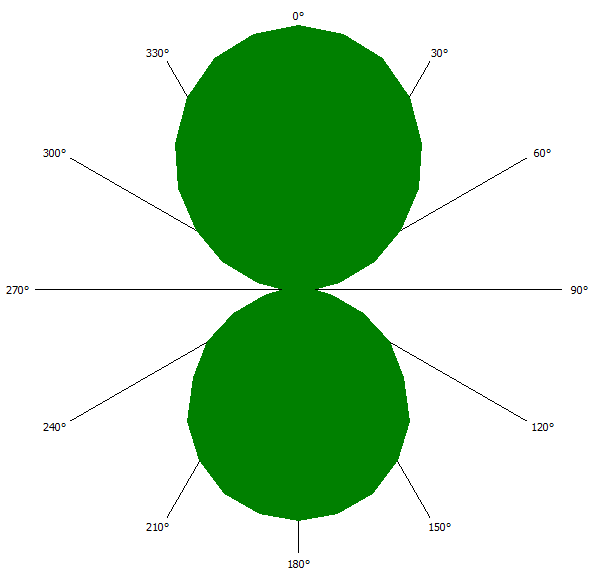
\includegraphics[width=0.3\textwidth]{2.3.3/6mmPolar/323_Polar_L1M-1Amp_freq3519_864.png} \label{6-m1mmDegeneracy}}
%		\quad
%		\subfloat[$\ell=1$, $m=0$ resonance]{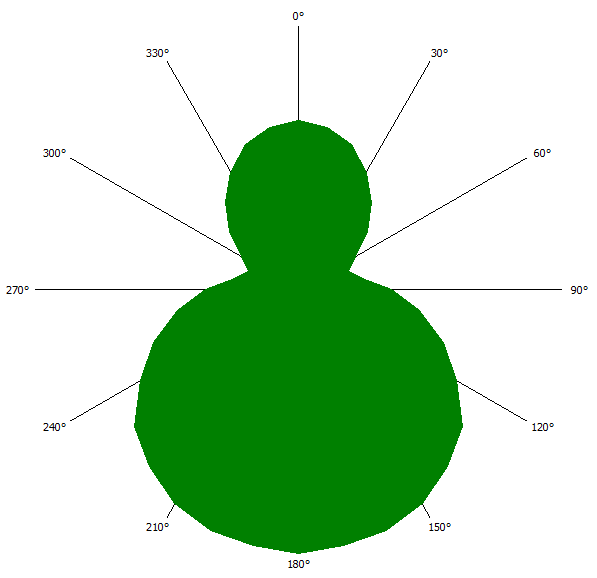
\includegraphics[width=0.3\textwidth]{2.3.3/6mmPolar/323_Polar_L1M0Amp_freq3534_956.png} \label{6-0mmDegeneracy}}
%		\quad
%		\subfloat[$\ell=1$, $m=1$ resonance]{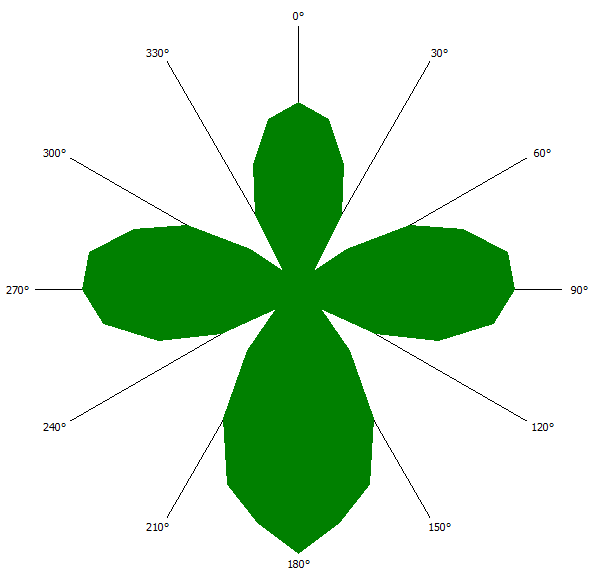
\includegraphics[width=0.3\textwidth]{2.3.3/6mmPolar/323_Polar_L1M1Amp_freq3632_422.png} \label{6-1mmDegeneracy}}
%		\caption{Polar plots of lifted degeneracies for 6mm spacing.}
%		\label{6mmliftedDegeneracy}
%	\end{figure}
%	
%	
%		Further, we focus on the \red{$\ell=2$} resonance and apply the spacing rings again to see how the peak splits.
%	
%	\begin{figure}[H]
%		\centering
%		\subfloat[Lifted degeneracy spectrum for $\ell=2$ 3mm spacing]{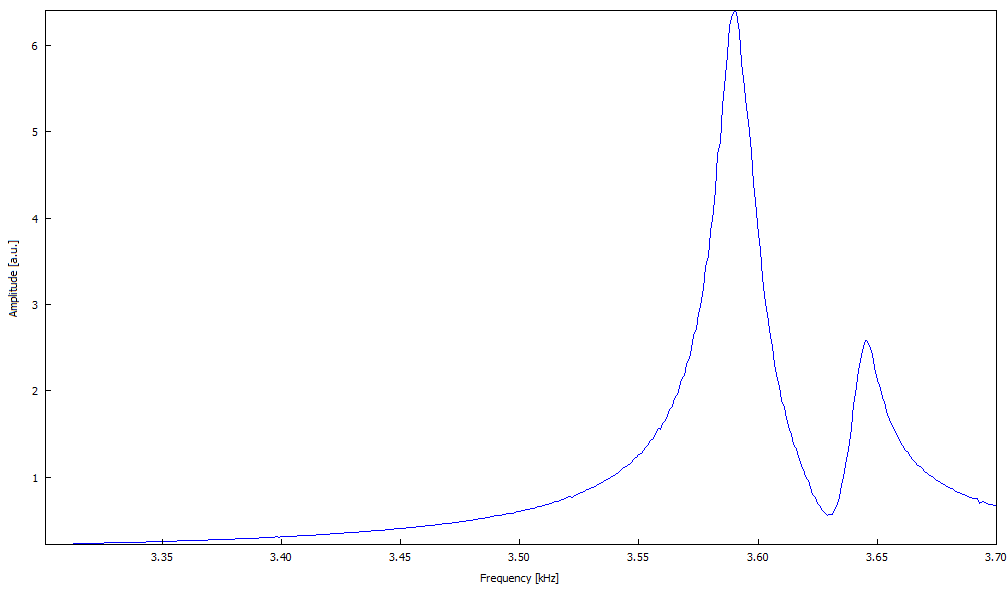
\includegraphics[width=0.3\textwidth]{2.3.3/323a180L13mmHires.png} \label{3mmDegeneracySpectrum}}
%		\quad
%		\subfloat[Lifted degeneracy spectrum for $\ell=2$ 6mm spacing]{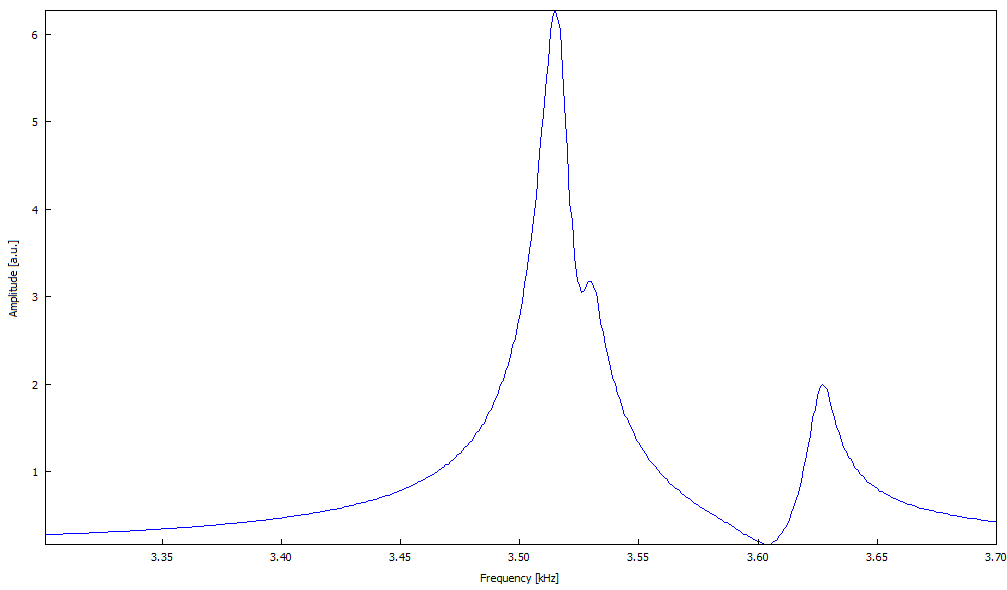
\includegraphics[width=0.3\textwidth]{2.3.3/323a180L16mmHires.png} \label{6mmDegeneracySpectrum}}
%		\quad
%		\subfloat[Lifted degeneracy spectrum for $\ell=2$ 9mm spacing]{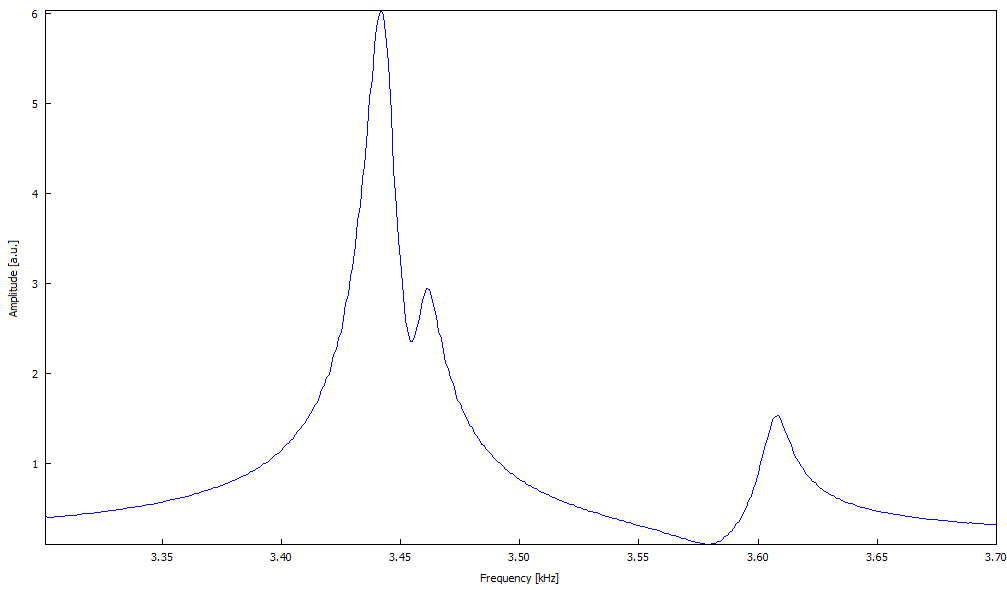
\includegraphics[width=0.3\textwidth]{2.3.3/323a180L19mmHires.png} \label{9mmDegeneracySpectrum}}
%		\caption{Progression of lifted degeneracies for the \red{$\ell=2$} state.}
%		\label{liftedDegeneracySpectrum}
%	\end{figure}



\end{document}